\title{%
  \Huge{\textbf{Interactive Tool for Teaching Hindley-Milner Type Inference through Visualisation}}
  \\
  \Large{Final report\\~\\~\textbf{Adam Jones}\\~Department of Computer Science\\~University of Warwick}
}

\documentclass[a4paper,fleqn,12pt]{article}

\usepackage[]{geometry}
\usepackage[utf8]{inputenc}
\usepackage[UKenglish]{babel}
\usepackage[UKenglish]{isodate}
\usepackage{amsmath}
\usepackage{amsfonts}
\usepackage{amssymb}
\usepackage{amsthm}
\usepackage{graphicx}
\usepackage{chngpage}
\usepackage{calc}
\PassOptionsToPackage{hyphens}{url}
\usepackage{hyperref}
\usepackage[nameinlink]{cleveref}
\usepackage{fancyhdr}
\usepackage{titletoc}
\usepackage[explicit]{titlesec}
\usepackage{natbib}
\usepackage[dvipsnames]{xcolor}
\usepackage[sc]{mathpazo}
\linespread{1.05} 
\usepackage[T1]{fontenc}
\usepackage{minted}
\usepackage{ragged2e}
\usepackage{adjustbox}

\hypersetup{
	colorlinks=true,
	linkcolor=black,
	urlcolor=black,
	citecolor=black
}

\definecolor{lightgrey}{rgb}{0.95,0.95,0.95}
\setminted{bgcolor=lightgrey}
\setmintedinline{bgcolor=lightgrey,escapeinside=||,mathescape=true}

\let\parencite\citep

\setlength{\parindent}{0mm}
\setlength{\parskip}{\medskipamount}
\renewcommand\baselinestretch{1.2}

\cleanlookdateon

\pagestyle{plain}
\renewcommand{\headrulewidth}{0.0pt}

\makeatletter
\fancypagestyle{plain}{
	\fancyhf{}
	\fancyhead[RE,RO]{\thepage}
	\fancyhead[LE,LO]{\textit{Interactive Tool for Teaching HM Type Inference through Visualisation}}
}
\makeatother

\begin{document}

\makeatletter
\begin{titlepage}

\LARGE \@title \\
\Large \\[1.5cm]

\vfill 

\begin{adjustwidth}{-\oddsidemargin-1in}{-\rightmargin}
  \centering
  
\includegraphics[width=\paperwidth]{line.png}
\end{adjustwidth}

\vspace*{-3.5cm}

\end{titlepage}
\makeatother

\pagestyle{plain}




TODO: Abstract
\section{Introduction}\label{id:h.6k9gcmunzldy}
Types are common features of many programming languages. Generally, types are bounds on program constructs (such as variables, expressions and functions) that limit what valid values they may take and how they should be interpreted within the program, however different languages use types differently. Most type systems include primitive data types such as integers, booleans and characters as well as composite types such functions from one type to another and lists of a type.

Type checking is the process by which a language’s compiler or interpreter validates that a program obeys the rules of the language’s type system. When a violation is detected, such as providing a boolean to a function accepting an integer, a type error is raised.

Type checking is primarily used to catch bugs in program code, preventing unexpected behaviour. A simple example of this is function application: functions’ types specify how they can be called which ensure some pre-conditions are met, such as the arguments being of an expected type. This allows function implementers to safely assume the data is of that type, and prevents function users calling the function with invalid arguments.

Type checking can happen either at compile time (static type checking) or runtime (dynamic type checking).

Compile-time type checking prevents many type errors from occurring at runtime. This is particularly useful when code paths may not be well tested or frequently used, as runtime checks only surface type errors when the problematic code is executed. Additionally, knowing types at compile-time allows for better tooling that improves developer productivity. For example, IDEs may use type information to suggest and perform automated refactorings \citep{ref1}, automatically generate documentation \citep{ref2} and autocomplete statements \citep{ref3}.

Compile-time type checking requires the program code to have enough information to validate its type safety. This may be in the form of type annotations or typed variable and function declarations. However, specifying types manually can be time-consuming and potentially difficult as it is additional work for the programmer, and large composite types can be especially difficult to determine and tedious to repeatedly write.

A type inference algorithm for a programming language’s type system can determine types automatically, which improves productivity by allowing programmers to get the best of types without having to explicitly specify them. Because of this, type inference is used in many popular programming languages with expressive type systems including Haskell, Rust and TypeScript.

An understanding of type inference would help computer scientists write cleaner code and debug type errors. However, few universities have core modules on type systems (although they may be touched on in programming curriculums) and there are limited easy-to-understand teaching resources on type inference. Therefore, many computer science graduates will be missing a useful understanding of how type inference actually works.

The goal of this project is develop a system to visualise the type inference process, with the aim of improving undergraduate students’ knowledge about it.

To achieve this, we develop a teaching resource that explains how type inference algorithms work for functional languages. An interactive web application allows students to enter expressions and view the results of a type inference algorithm, along with the steps taken to get to that result. This is particularly useful in the context of modules teaching functional languages such as Haskell which perform similar type inference.
\subsection{Related work}\label{id:h.2mwaav7jkal4}
There have been previous attempts to build visualisation and teaching tools related to type systems.

{\centering \begin{figure}[h!]
  \centering
  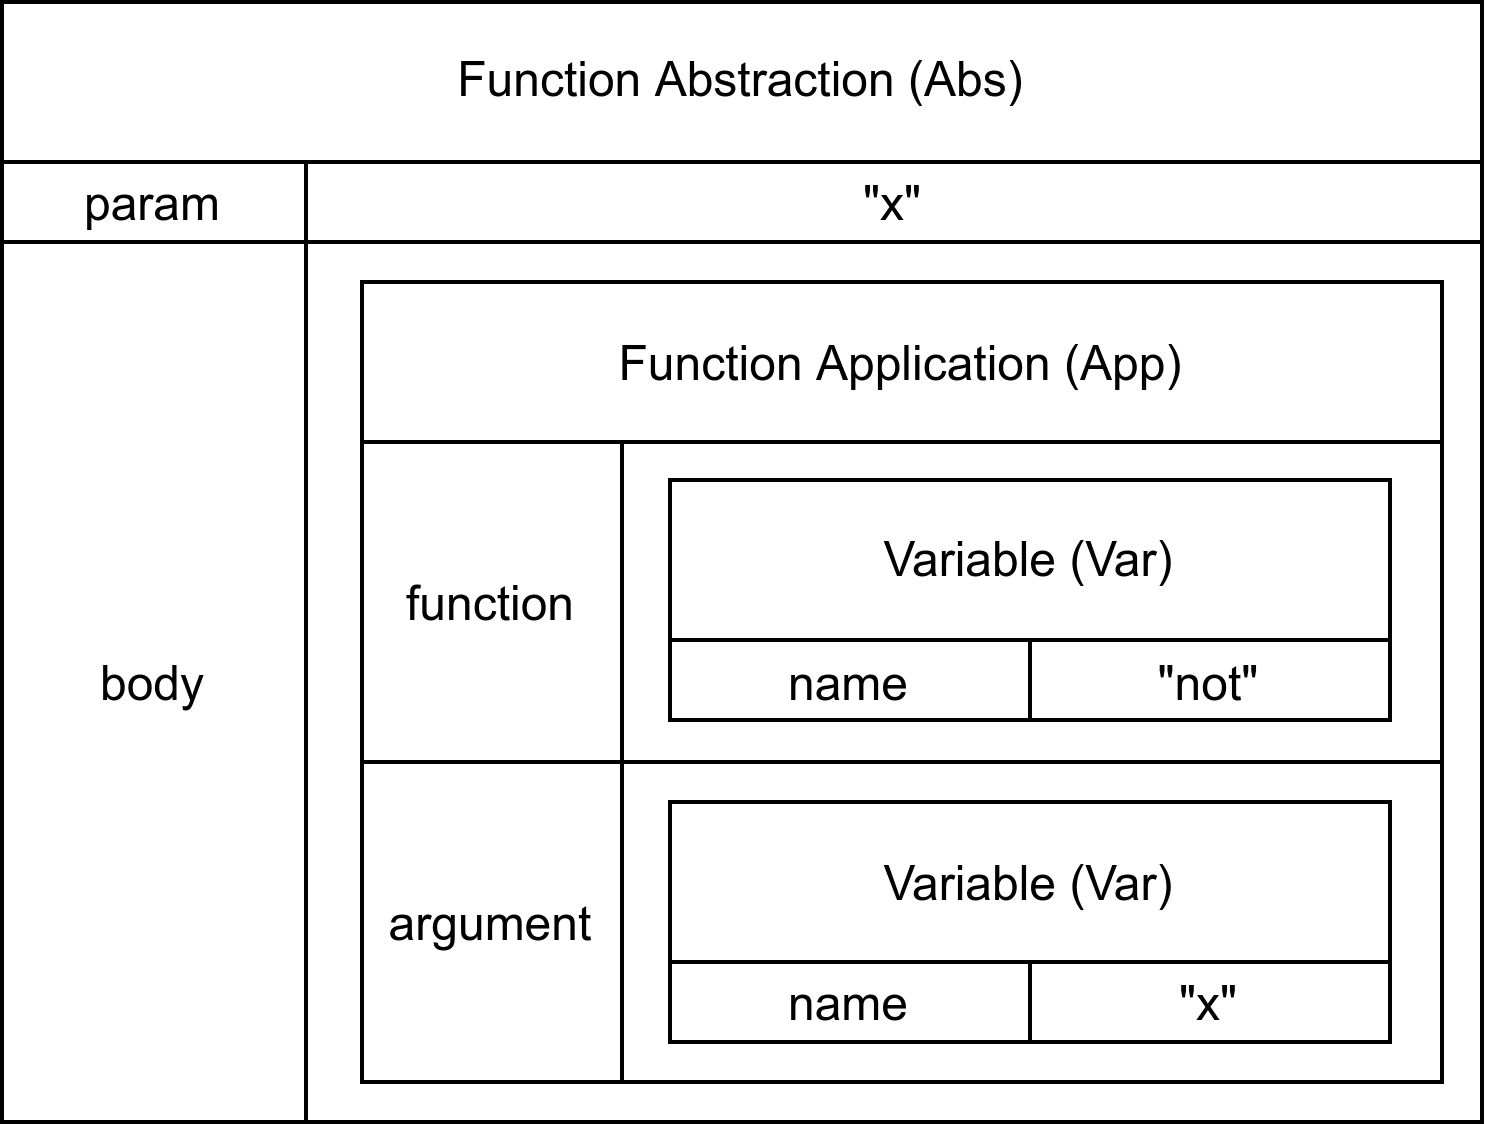
\includegraphics[width=0.770\linewidth]{images/image19.png}
  \caption{Screenshot of results from TypeTool, taken from their paper}
\end{figure} \par}

One example is TypeTool by~\cite{ref4}, which visualises type inference through a web application. Users enter an expression in a custom expression language, submit a request to a server and are redirected to a page displaying an initial syntax tree, a final syntax tree and an overall substitution. By allowing users to enter their own expressions, students can explore how the systems work in different cases to gain an intuitive understanding of the concepts.

TypeTool’s authors found in teaching the University of Porto’s functional programming course that the tool was “especially useful for students, because it helps to understand the type systems of the most common typed functional languages” and that “[presenting] the basis of type inference technology [...] significantly improved the way students deal with type errors because they understand the type system.”

However, TypeTool’s parsing and type inference is done server-side so there is a delay between the user entering an expression and seeing the result. While short, a delay reduces the ease-of-use and may discourage users from trying many different expressions. Both delayed feedback and the lack of step-by-step explanations reduce learning quality \citep{ref5}, particularly in the area of rule learning.~\cite{ref6} showed that immediate explanatory feedback is most effective at learning how to apply rules in computer programming. It also lacks step-by-step explanations, and it is unclear whether it supports processing incorrectly-typed expressions.

In addition, the tool is now inaccessible as the server hosting the application is no longer running and the source code has not been published.

Another tool in the area of visualising type systems was developed by~\cite{ref7}. It is a visual functional programming system which shows types during function application for a subset of Standard ML, used to teach first year undergraduate students. However, this did not explicitly show the type inference process and as a desktop application rather than web app it is less accessible to lecturers and students. It also didn’t support key functional language constructs such as function declarations and let bindings, and required significant explanation before using the tool to understand its output.

{\centering \begin{figure}[h!]
  \centering
  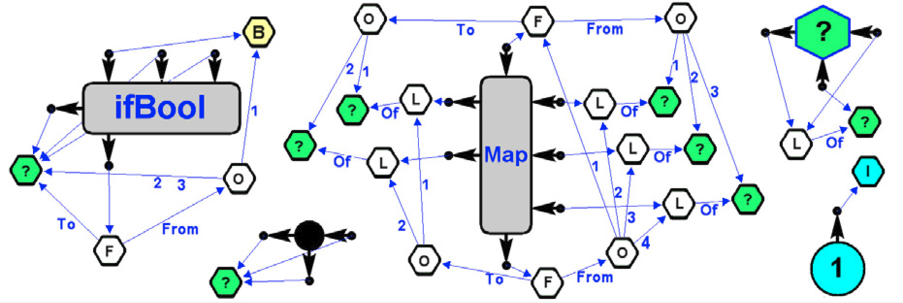
\includegraphics[width=0.797\linewidth]{images/image3.png}
  \caption{Screenshot of Yung and Michaelson's tool, taken from their paper}
\end{figure} \par}

NiMo \citep{ref8} is a graphical programming language related to functional data processing which allows users to reason about the flow of data through a program. The types of data and processes can be inspected in NiMoToons, and type inference is performed over the network of components. However, larger expressions can become complicated and be difficult to interpret. While NiMo performs type inference internally it is not a key focus to the end-user, and as such does not explain its steps. Additionally, it is harder to relate back to more commonly used, textual functional languages like Haskell.

{\centering \begin{figure}[h!]
  \centering
  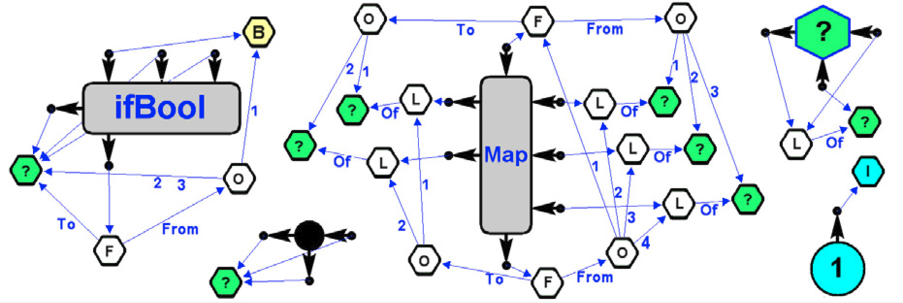
\includegraphics[width=0.960\linewidth]{images/image16.png}
  \caption{A diagram showing the types of some variables in NiMo, taken from their paper}
\end{figure} \par}

\cite{ref9} implemented a successful teaching tool, named TILC, for visualising lambda-calculus parse trees in order to help with teaching lambda-calculus to undergraduate students. They noted that to develop an intuitive understanding, students would benefit from experimenting with lambda-calculus and that “a tool that deals with all these aspects in a friendly and graphical manner incentivises [experimentation]”. TILC was successful, with the module organisers of ‘programming paradigms’ at the Universitat de Girona having a “good experience of using this tool in the course lectures and as a downloadable tool for students”. The authors suggested extending TILC to show types and type inference would have pedagogical value.

To summarise, types aid the construction of correct programs and type checking can detect issues in programs, either at compile-time or runtime. Type inference is a method often used alongside compile-time type checking to determine types in a program, an understanding of which could benefit computer scientists in writing and debugging programs. Some solutions exist which give students a better idea about types, however they either have significant limitations or do not explicitly cover type inference. In this report, we present an interactive web application for teaching type inference.
\section{Background}\label{id:h.ebjyqi73zdyo}
\subsection{$\lambda$-calculus}\label{id:h.odw4vku9eizz}
A $\lambda$-calculus is a representation of computation. The first $\lambda$-calculus set out by~\cite{ref10}, often viewed as the canonical $\lambda$-calculus, simply has variables, function abstraction and application.

For this project, we will consider a calculus with five constructs to build expressions from. As a formal grammar:

\begin{figure}[h!]
  \centering
  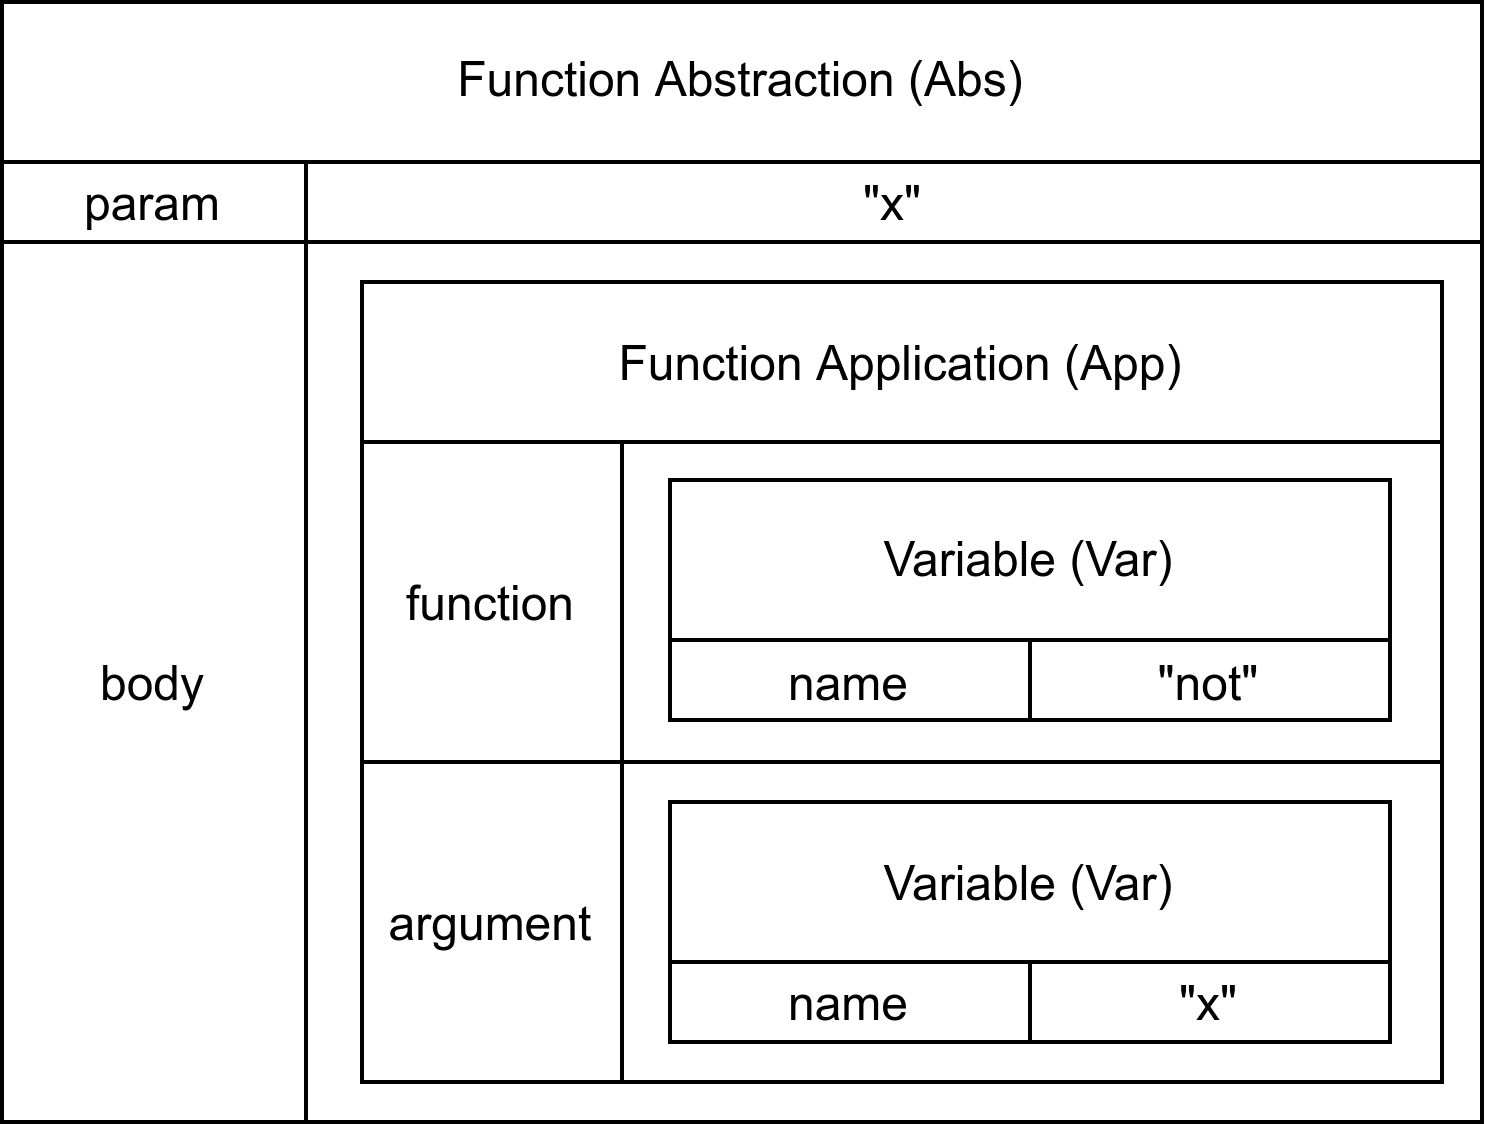
\includegraphics[width=0.510\linewidth]{images/image18.png}
\end{figure}
    | c constant

TODO: latex-ify the above, move constant to top

For example, consider the expression \mintinline{text}{|($\lambda$x. x) y|}

It has variables \mintinline{text}{|x|} and \mintinline{text}{|y|}. Variables may be bound or free (unbound). Here \mintinline{text}{|x|} is bound as it is a parameter in the function abstraction, and \mintinline{text}{|y|} is free as there is nothing which binds it. This can be thought of in a similar way to how variables in most imperative programming languages have a scope where they are defined or undefined.

The function abstraction mentioned is the \mintinline{text}{|$\lambda$x. x|} part. This defines an anonymous function which given an argument (before the full stop) \mintinline{text}{|x|} simply returns (after the full stop) \mintinline{text}{|x|}, i.e. the identity function. A function to add three to an input might be written \mintinline{text}{|$\lambda$x. x + 3|} (although many of the most fundamental $\lambda$-calculi do not have such explicit notions of addition or numbers).

Functions may be returned by other functions, which enables functions to have the appearance of taking multiple arguments. For example \mintinline{text}{|$\lambda$x. ($\lambda$y. x)|} can be viewed as a function which takes two arguments and returns the first one, even though really it is a function taking one argument which returns a function taking another argument for a result. Here explicit brackets have been given for clarity, but they aren’t necessary. Additionally, sometimes multiple arguments like this are written together, so \mintinline{text}{|$\lambda$x. ($\lambda$y. x)|}, \mintinline{text}{|$\lambda$x. $\lambda$y. x|} and \mintinline{text}{|$\lambda$xy. x|} all mean the same thing.

Finally, the function application is actually applying the function \mintinline{text}{|$\lambda$x. x|} to the argument \mintinline{text}{|y|}. In $\lambda$-calculus evaluation is performed via $\beta$-reductions. In our example this could be done by substituting the argument \mintinline{text}{|y|} for parameter \mintinline{text}{|x|} in the body of the function \mintinline{text}{|x|}, resulting in \mintinline{text}{|y|}:

This expression’s construction can be represented as an abstract syntax tree:

TODO: tree diagram of the expression

In addition to these three constructs, the \mintinline{text}{|let|} construct allows binding a value to a variable in an expression. For example \mintinline{text}{|let x = 3 in x + x|} binds \mintinline{text}{|x|} to the value \mintinline{text}{|3|} in \mintinline{text}{|x + x|}.

A \mintinline{text}{|con|} construct is added to represent literal constants, such as numbers or booleans like \mintinline{text}{|3|} and \mintinline{text}{|True|}.

$\lambda$-calculi have been extensively studied, often using formal inductive definitions. For example, the inductive definition for the set of free variables (\mintinline{text}{|var|}s not bound by function abstraction or let statements) is:
\begin{itemize}
  \item \mintinline{text}{|con|}: $FV(c) = \varnothing$
  \item \mintinline{text}{|var|}: $FV(x) = \{ x \}$
  \item \mintinline{text}{|app|}: $FV(e\_1 e\_2) = FV(e\_1) \cup FV(e\_2)$
  \item \mintinline{text}{|abs|}: $FV(\lambda x. e) = FV(e) - \{ x \}$
  \item \mintinline{text}{|let|}: $FV(let x = e\_1 in e\_2) = FV(e\_2) - \{ x \}$
\end{itemize}
where e is an expression.

TODO: fix latex of above

Given these rules the set of free variables for any combination of these constructs can be determined. This can be demonstrated for our example expression \mintinline{text}{|($\lambda$x. x) y|}, which is shown in a tree structure below. More generally this is an example of how an inductive definition can tell us something about the entire program which is how some type inference algorithms can be viewed.

TODO: tree diagram of the expression with the sets of free variables at each node.

Most real-world environments define a context which binds some variables by default to in-built values. For example Haskell’s GHC primitives and Prelude includes basic variables like \mintinline{text}{|[]|} (the empty list) and \mintinline{text}{|not|} (a function which inverts booleans). These can be considered bound at the top level and removed from the set of free variables there.
\subsection{The simply typed $\lambda$-calculus}\label{id:h.w7vj0r89b86n}
Typed $\lambda$-calculi extend the system with the concept of types.

The simply typed $\lambda$-calculus is one of the simplest typed $\lambda$-calculi, and introduced by~\cite{ref11} is often viewed as the canonical typed $\lambda$-calculus. It has the \mintinline{text}{|var|}, \mintinline{text}{|abs|}, \mintinline{text}{|app|} and \mintinline{text}{|con|} constructs. Types in this system are either base types (often in the literature Greek letters $\alpha$, $\beta$, $\gamma$ are used, but these can be thought of similar to numbers, booleans, characters etc.) or functions between other types (such as \mintinline{text}{|Int \rightarrow Bool|}, or \mintinline{text}{|Int \rightarrow (Bool \rightarrow Bool)|}).

The syntax adds type annotations to \mintinline{text}{|var|}, \mintinline{text}{|abs|} and \mintinline{text}{|con|} constructs, for example ($\lambda$x: Int. odd\textsuperscript{Int \rightarrow Bool} x\textsuperscript{Int}) 3\textsuperscript{Int} (although often for simplicity the types of \mintinline{text}{|var|} and \mintinline{text}{|con|} subexpressions, those in superscript, are left out).
\subsection{Hindley-Milner type system}\label{id:h.gsouq2axz3k}
Hindley-Milner (HM) is a typed $\lambda$-calculus which allows for the types of programs to be inferred and no type annotations are required \citep{ref12,ref13}. It extends the simply typed $\lambda$-calculus by adding \mintinline{text}{|let|} bindings and a richer type system that includes \textit{type functions} and \textit{polymorphism}.

Like expressions, types can be considered to be built from \mintinline{text}{|var|} variables and \mintinline{text}{|app|} function applications. Type variables are either base types like \mintinline{text}{|Bool|} and \mintinline{text}{|Int|} or type functions. Type functions can be applied, taking types as parameters to construct composite types.

\begin{figure}[h!]
  \centering
  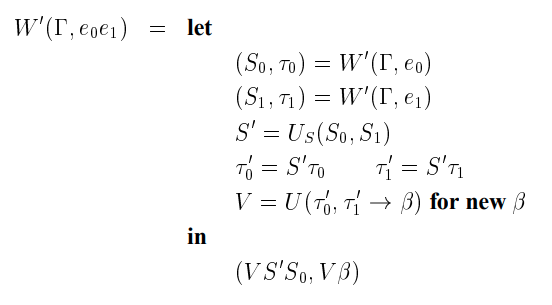
\includegraphics[width=0.467\linewidth]{images/image11.png}
\end{figure}
where C is a set of type functions such as \mintinline{text}{|->|}, \mintinline{text}{|List|} and \mintinline{text}{|Maybe|}.

TODO: latexify the above, replace alpha with tn

For a type to be valid all functions must be fully applied, unlike expressions where the final expression may be a function. As with expressions, we can again assume a global context that binds the basics variables like \mintinline{text}{|Bool|} and \mintinline{text}{|Int|}. In Hindley’s original paper only \mintinline{text}{|->|} was considered as a type function (i.e. $C = \{ \rightarrow \}$), however here we explore several type functions that have been found useful in practice.

The type function we’ve already been using is \mintinline{text}{|->|} (the \textit{function} type function). It takes two types as arguments and represents a function from the first type to the second. A function from \mintinline{text}{|Int|} to \mintinline{text}{|Bool|} is represented by \mintinline{text}{|(->) Bool Int|} in prefix notation, although would more commonly be written infix as \mintinline{text}{|Bool \rightarrow Int|}.

The function type function (\mintinline{text}{|->|}) should not be confused with the function type: an expression representing a function has a function type, and that function type is the function type function applied to arguments. For example \mintinline{text}{|$\lambda$x. x + 3|} has a function type \mintinline{text}{|Int \rightarrow Int|}, which is the function type function \mintinline{text}{|->|} applied to arguments \mintinline{text}{|Int|} and \mintinline{text}{|Int|}.

The list type function is also very common, which given one type argument represents a list of those types. A list of booleans might be written \mintinline{text}{|List Bool|} or \mintinline{text}{|[] Bool|} in prefix notation, although often the list type is represented by wrapping the type argument in square brackets instead like \mintinline{text}{|[Bool]|}.

\mintinline{text}{|Maybe|} is another type function commonly used in functional languages like Haskell. A \mintinline{text}{|Maybe|} represents the optional presence of something, similar to Java’s \mintinline{text}{|Optional|} and C++’s \mintinline{text}{|std::optional|}. Applied to a boolean type this may be written \mintinline{text}{|Maybe Bool|}, representing a wrapper around nothing or a boolean. In Java this would be represented with a generic as \mintinline{text}{|Optional<Boolean>|} and in C++ as \mintinline{text}{|std::optional<bool>|}.

A similar common type function is \mintinline{text}{|Either|}, which takes two type arguments and represents a wrapper around either one of the types. For example, an either for a boolean or integer is written \mintinline{text}{|Either Bool Int|}.

Finally, tuples represent a defined-length sequence of elements of specific types. Tuple constructors are a set of type functions representing a cross product of their type arguments, named \mintinline{text}{|,|}, \mintinline{text}{|,,|}, \mintinline{text}{|,,,|} and so on for different element lengths. A 3-tuple holding a boolean, integer and integer can technically be written in prefix notation as \mintinline{text}{|(,,) Bool Int Int|} but instead generally tuples borrow mathematical syntax with parentheses and commas like \mintinline{text}{|(Bool, Int, Int)|}.

The set of types made from \mintinline{text}{|var\_t|} and \mintinline{text}{|app\_t|} are known as monotypes. For example, \mintinline{text}{|Bool|}, \mintinline{text}{|Int|}, \mintinline{text}{|Bool \rightarrow Int|}, and \mintinline{text}{|Bool \rightarrow [(Bool, Int \rightarrow Maybe Bool)]|} are all monotypes.

Adding zero or more for-all quantified type variables to monotypes forms polymorphic types or polytypes (called principal type schemes by Hindley). This can be thought of as the \mintinline{text}{|abs|} equivalent for types, written as \mintinline{text}{|\forall a. \rho|} where \mintinline{text}{|\rho|} is a polytype. This definition makes monotypes a special case of polytypes: monotypes are polytypes with zero for-all qualified type variables. We can therefore consider ‘type’ to mean ‘polytype’. By convention, we use $t0, t1, t2, \dots$ for free type variables, and $a, b, c, \dots$ for for-all quantified type variables.

\begin{figure}[h!]
  \centering
  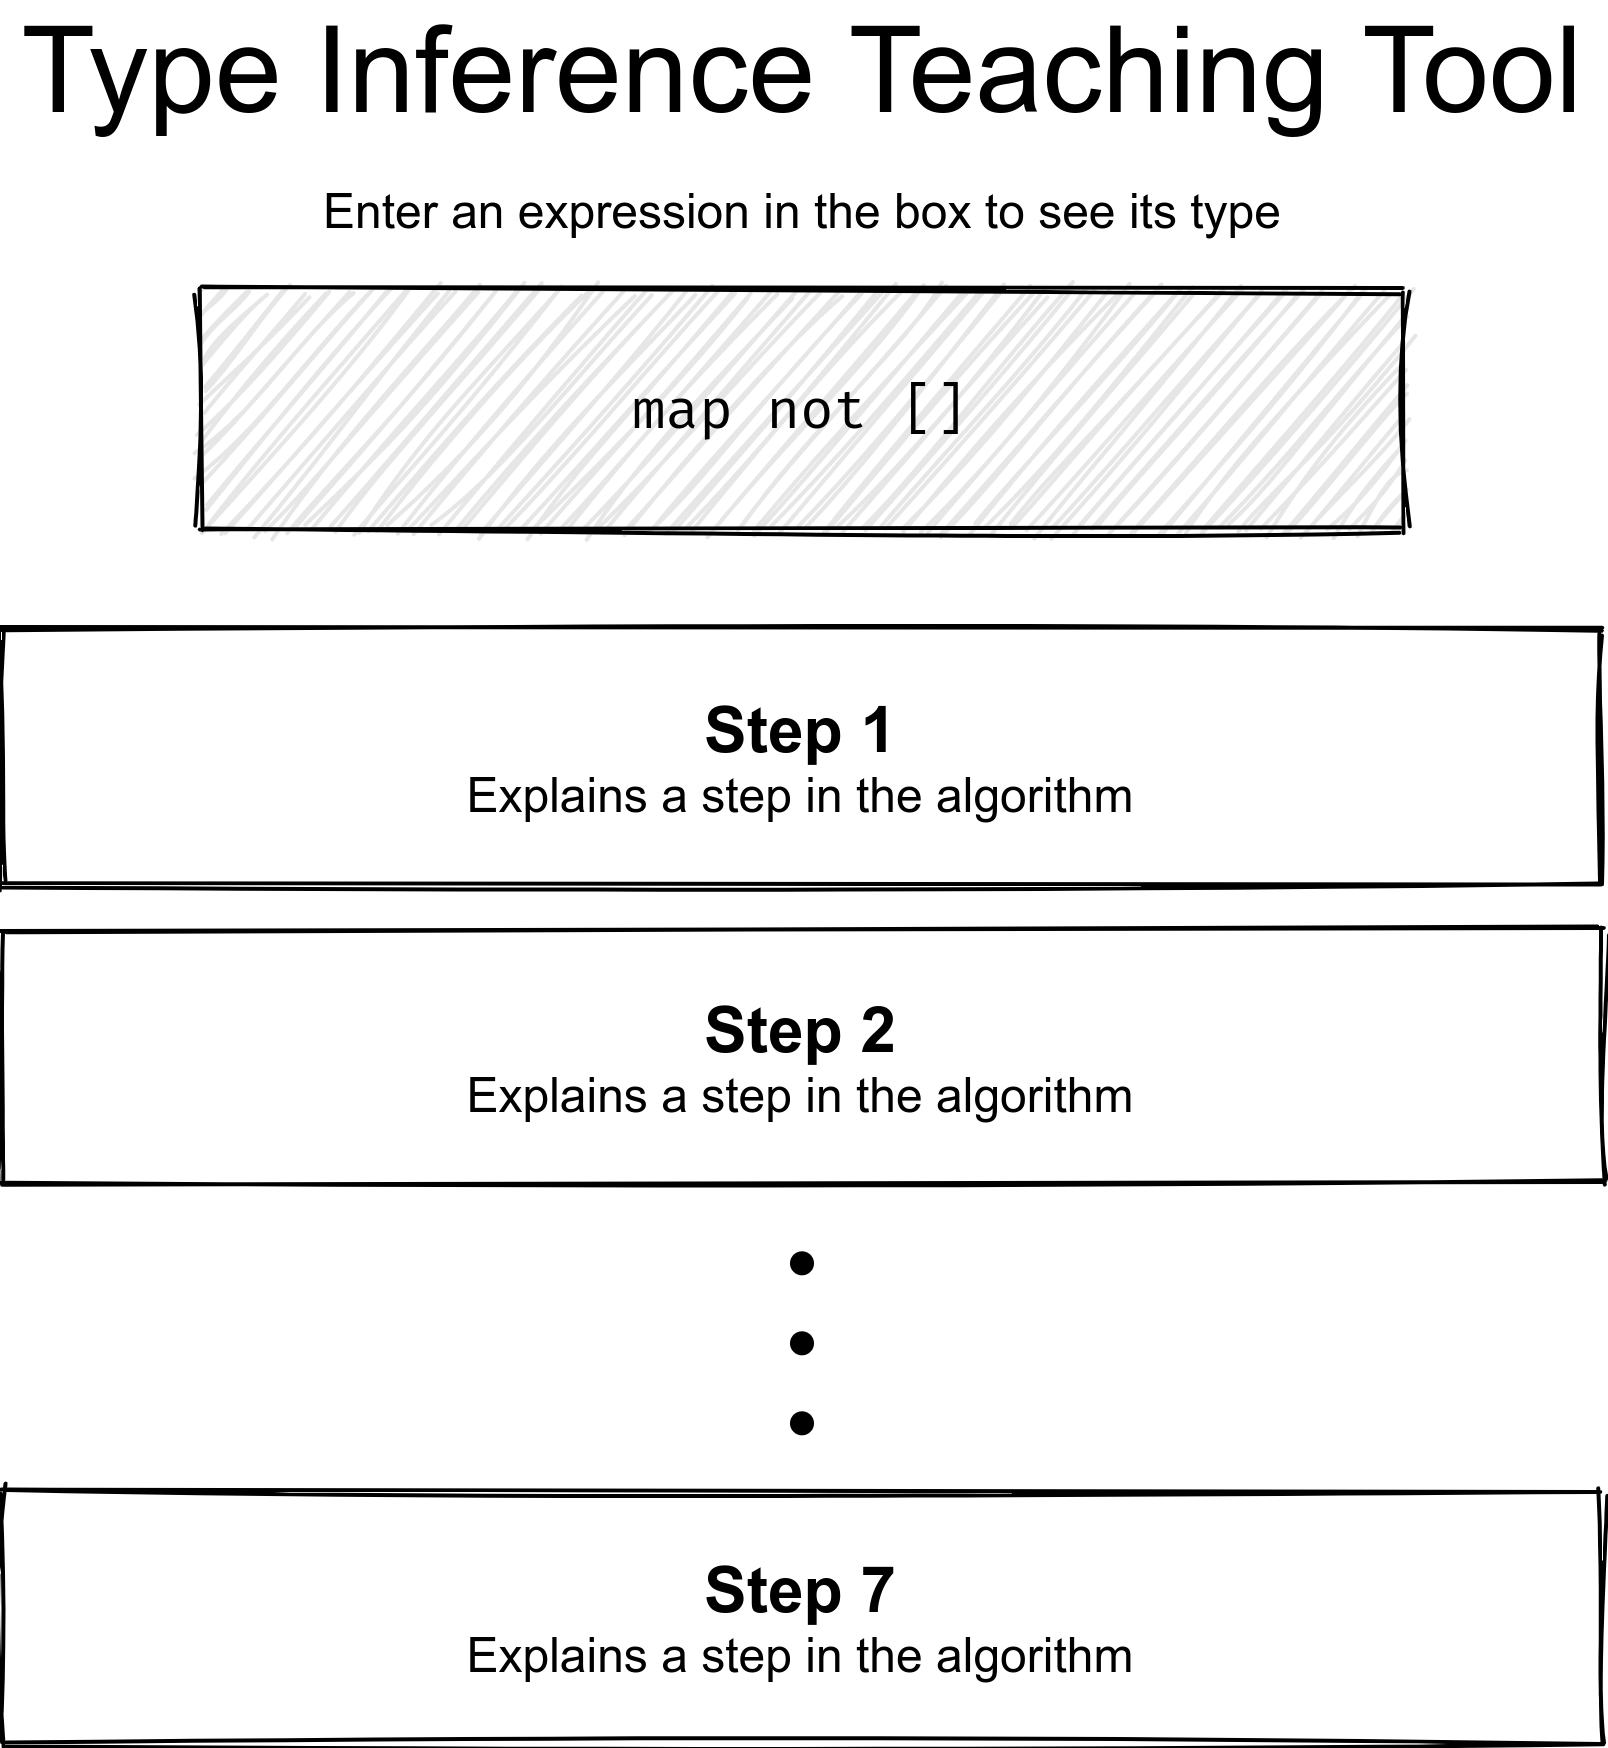
\includegraphics[width=0.290\linewidth]{images/image20.png}
\end{figure}

TODO: latexify the above, but use rho instead of sigma and a instead of alpha

Polytypes allow for parametric polymorphism, where a type may be parameterized by a for-all bound quantifier. This allows functions to accept different types as long as they meet certain constraints. For example the \mintinline{text}{|length|} function is polymorphic: it has the polytype \mintinline{text}{|\forall a. [a] \rightarrow Int|}, which accepts a list of any type and returns its length as an integer. It accepts different types such as \mintinline{text}{|[Bool]|} and \mintinline{text}{|[Int]|} as both of these meet the constraint of being a list.

Correctly inferring polymorphic types can be difficult, and in fact~\cite{ref14} proved that doing so for System F, a type system similar to Hindley-Milner with fewer typing rule constraints, is undecidable. To prevent undecidability, HM avoids overusing polytypes, using only monotypes for \mintinline{text}{|var|}, \mintinline{text}{|con|}, \mintinline{text}{|app|} and \mintinline{text}{|abs|} expressions.

To allow for some polymorphism, \mintinline{text}{|let|} expressions’ parameters are polymorphic in the \mintinline{text}{|let|} body. The process by which the monomorphic parameter type is turned into a polymorphic one is known as generalisation. The overall type of \mintinline{text}{|let|} expressions themselves are not generalised.

This is the difference between:
\begin{itemize}
  \item \mintinline{text}{|let i = (\lambda x \rightarrow x) in (i 3, i True)|} type-checks, as i is generalised to the polytype \mintinline{text}{|\forall a. a \rightarrow a|} within the body \mintinline{text}{|(i 3, i True)|} so can be applied to both an \mintinline{text}{|Int|} and \mintinline{text}{|Bool|}
  \item \mintinline{text}{|(\lambda i \rightarrow (i 3, i True)) (\lambda x. x)|} does not type-check as the function abstraction \mintinline{text}{|(\lambda x. x)|} has the monotype \mintinline{text}{|t0 \rightarrow t0|}, and \mintinline{text}{|t0|} must take only one type in both tuple parts - it cannot be both an \mintinline{text}{|Int|} and a \mintinline{text}{|Bool|}.
\end{itemize}

Hindley-Milner is the basis for the type system of Standard ML \citep{ref15} (which OCaml and F\# are related to) and was the basis of the type system in Haskell \citep{ref16}. It has influenced the development of Rust and Swift, and more generally type inference is present in many more languages including Java, JavaScript and C++.

Haskell has since been extended with type-class constraints \citep{ref17}, functional dependencies \citep{ref18}, and generalised algebraic data types (GADTs) \citep{ref19}. Haskell’s inference engine was moved onto a new engine, OutsideIn(X), when GHC 7.2 was released November 2011 after~\cite{ref20} proposed a solution to the issues with Hindley-Milner’s poor performance on large programs and difficulty inferring expressions without principal types that arise with type-class constraints and GADTs. In doing this, Haskell stopped automatically generalising variables bound by \mintinline{text}{|let|} expressions after~\cite{ref21} argued that generalising \mintinline{text}{|let|} bindings is complex in type inference engines other than HM and the feature was rarely used in practice, with the change only affecting 0.13\% lines of the GHC core libraries. This change does however take it further away from performing HM-like type inference.

Rust’s compiler, rustc, did at one time use a variant of HM for type inference. However,~\cite{ref22} proposed a new scheme which was later implemented to simplify how the compiler reasoned about types. Similarly to Haskell’s move to OutsideIn(X), the new type inference reduces flexibility in some edge cases, although practically this is rare. Both rustc and Rust’s core libraries compiled under the new type inference scheme without changes. Later on,~\cite{ref23} developed chalk, a library designed to be used in rustc to help implement Rust’s generics. This library makes heavy use of unification, a key component of many HM type inference algorithms.

Apple’s Swift heavily uses type inference. It is implemented using a “constraint-based type checker that is reminiscent of the classical Hindley-Milner type inference algorithm” \citep{ref24}. Like other languages it extends HM with additional language features, such as more expressive polymorphic types with additional constraints. To adapt HM to a procedural language, and for improved performance and better error messages, Swift limits type inference to individual statements rather than entire programs.

In addition to their own inference engines, many languages allow the programmer to add more type information through explicit type annotations or casting. This is particularly helpful where the programmer knows more than the type inference algorithm about the limits on how a part of a program will be used.

Java allows casting objects and TypeScript has its \mintinline{text}{|as|} type assertion operator. Programmers can use these sparingly (and often in combination with \mintinline{text}{|instanceof|} and \mintinline{text}{|typeof|} operators respectively) as an escape hatch to work around the type inference algorithm’s limitations. In these situations statements may not be able to be type checked at compile-time so instead runtime checks are performed to maintain type safety.

Java allows casting an object to a subclass \citep{ref25}. Runtime checks are performed, which throw a \mintinline{text}{|ClassCastException|} in case the object is not actually an instance of the subclass.

\begin{minted}[breaklines]{java}
// Dog and Cat extend Animal

Animal c1 = new Dog();
Dog s1 = (Dog) c1; // okay

Animal c2 = new Cat();
Dog s2 = (Dog) c2; // throws ClassCastException at runtime
\end{minted}

TypeScript allows for casting compatible objects with its \mintinline{text}{|as|} operator, or overriding the compile-time type checking completely with a \mintinline{text}{|@ts-ignore|} comment. The following shows that some type-safe code is rejected by the TypeScript type checker, but with several possible workarounds.

\begin{minted}[breaklines]{typescript}
const a = Math.random() < 0.5 ? 'cs310' : 310; // has type "cs310" | 310
const b = a + a; // throws a type error, but b could have type "cs310cs310" | 620

const c = a == 'cs141' ? a + a : a + a; // okay, has type number | string
const d = a as any + a; // okay, has type any
const e = a as any + a as 'cs310cs310' | 620 // okay, has type "cs310cs310" | 620
// @ts-ignore
const f: 'cs310cs310' | 620 = a + a; // okay, has type "cs310cs310" | 620
\end{minted}

TODO: (maybe?) Add section on TypeScript/Elm?

\underline{\href{https://aaltodoc.aalto.fi/bitstream/handle/123456789/42719/master\_Mikkonen\_Juuso\_2020.pdf}{https://aaltodoc.aalto.fi/bitstream/handle/123456789/42719/master\_Mikkonen\_Juuso\_2020.pdf}}
Talks about statically typed languages in JavaScript-land. Mentions things like TypeScript don’t use HM because JS has a lot of structural typing (i.e. if objects have the right properties it’s fine to call methods that depend on that interface) and subtyping.

While real-world languages don’t work exactly like HM, for the purposes of the teaching tool HM gives a good representation of how type inference works to students. HM avoids being too complex to understand, and is still related to how languages commonly used in practice perform type inference.
\subsection{Hindley-Milner type inference}\label{id:h.admfqf7bhkct}
Various algorithms are available to infer types in Hindley-Milner such as Algorithm W by~\cite{ref26} and Algorithm M by~\cite{ref27}. Algorithm W takes a bottom-up approach, attempting to infer the types of subexpressions up the abstract syntax tree, while Algorithm M takes a top-down approach, inferring types down the tree. Algorithm W’ is a minor extension to Algorithm W, by~\cite{ref28} which can improve the quality of type errors raised.

Substitutions are a key concept from logic used by the algorithms. These are maps from variables to terms. When applied to an expression, the variables are substituted with their corresponding terms. In the case of type inference, the variables are type variables, the terms are monotypes and expressions are types.

TODO: fix this latex

Substitutions are represented with curly braces, with each entry separated by a comma and the variables and terms separated with an arrow. For example, $\{ t0 \mapsto t1, t2 \mapsto (Int, Bool) \}$ would replace $t0$ with $t1$, and replace $t2$ with $(Int, Bool)$. Applied to the type $t0 \rightarrow t1 \rightarrow t2$ results in $t1 \rightarrow t1 \rightarrow (Int, Bool)$.

When applying substitutions replacements are performed simultaneously, meaning each variable in the expression may be mapped at most once. For example the substitution $S = \{ t0 \mapsto t1, t1 \mapsto t2 \}$ applied once to the expression $t0$, as $S(t0)$ results in $t1$, not $t2$. Applying the substitution twice, $S(S(t0))$ would result in $t2$.

Any number of substitutions may be applied to expressions. For example, given $S\_1 = \{ t0 \mapsto t2, t1 \mapsto t3 \}$ and $S\_2 = \{ t0 \mapsto t1 \}$, we may apply both to an expression $t0$. Note that this is not commutative, $S\_1(S\_2(t0)) = t3$ while $S\_2(S\_1(t0)) = t2$.

Substitutions may be combined to have the same effect as applying them in order to an expression $E$. For example, with $S\_1 = \{ t0 \mapsto t2, t1 \mapsto t3 \}$ and $S\_2 = \{ t0 \mapsto t1 \}$ again, $combine(S\_1, S\_2)(\rho) = S\_1(S\_2(\rho)) = \{ t0 \mapsto t3, t1 \mapsto t3 \}(\rho)$. As application is not commutative, the order substitutions are combined in matters, i.e. $combine(S\_1, S\_2)$ does not necessarily equal $combine(S\_2, S\_1)$. Combining substitutions is however associative, as $combine(S\_1, combine(S\_2, S\_3))(\rho) = S\_1(S\_2(S\_3(\rho))) = combine(combine(S\_1, S\_2), S\_3)(\rho)$.

A substitution is said to unify two expressions if when applied to both it results in equal expressions. For example, $\{ t0 \mapsto Int, t1 \mapsto Bool \}$ unifies $(t0, Bool)$ and $(Int, t1)$, as when the substitution is applied to either expression the result is $(Int, Bool)$.

Unification is the process of finding unifying substitutions given two expressions, or reporting no such substitution exists.~\cite{ref29} presents a simple algorithm for unification, and~\cite{ref30} and~\cite{ref31} set out linear time unification algorithms.

In the type inference algorithms W, W’ and M, unification is applied to pairs of monotypes. This results in substitutions which effectively combine the various type constraints giving us a final type.

For example, take an expression satisfying two type constraints: it matches the monotype $[Bool] \rightarrow t0$ and it matches with the monotype $[t1] \rightarrow t1$. These constraints might arise in evaluating the type of \mintinline{text}{|head [True]|}. The first constraint is from knowing \mintinline{text}{|[True]|} is a $[Bool]$ so the function should accept a $[Bool]$. The second constraint is based on the known definition of \mintinline{text}{|head|} in the global context. Unification can find the unifying substitution $\{ t0 \mapsto Bool, t1 \mapsto Bool \}$, giving the overall type $[Bool] \rightarrow Bool$. We can then see the resultant type of \mintinline{text}{|head [True]|} is $Bool$.

If at any point unification is not possible, the type constraints must be incompatible and so a type error is raised. For example, there is no unifying substitution for $Int \rightarrow t0$ and $Bool \rightarrow t1$ as one is a function accepting an $Int$ and the other accepts a $Bool$.

For practical purposes, in type inference algorithms we require unifying substitutions to be finite as infinite types are difficult to represent and reason about. For example \mintinline{text}{|x|} in \mintinline{text}{|$\lambda$x. x x|} needs to be a function that accepts itself. Initially assuming \mintinline{text}{|x|} has type $t0 \rightarrow t1$ and knowing it should accept itself, it also has type $(t0 \rightarrow t1) \rightarrow t1$. It also must accept that, so has type $((t0 \rightarrow t1) \rightarrow t1) \rightarrow t1$, $(((t0 \rightarrow t1) \rightarrow t1) \rightarrow t1) \rightarrow t1$, and so on. This is an infinite type and is not allowed by HM. Note that this does not exclude functions from HM which do accept themselves, such as the identity function \mintinline{text}{|id|} with its finite type $\forall a. a \rightarrow a$, as long as they themselves have finite types.

Detecting infinite types in unification is done by checking whether the types are not equal and one of the types occurs in another. This is known as the occurs check. In the previous example \mintinline{text}{|$\lambda$x. x x|} we might try to unify $t0 \rightarrow t1$ with $t0$. $t0$ occurs in $t0 \rightarrow t1$ so there is no finite unifying substitution (an infinite unifying substitution is $\{ t0 \mapsto ((((t0 \rightarrow t1) \rightarrow t1) \rightarrow infinite t1s \dots) \rightarrow t1) \}$). The occurs check failing necessarily means we have an infinite type: the type contains itself.

Inferring types is done in a typing context. Languages often have a global context with built-in functions and their types pre-defined, such as Haskell’s Prelude and JavaScript’s global objects.

Typing contexts can be seen as maps from variable names to their corresponding types, and are represented with the symbol $\Gamma$. For example a context with some common functions may be written $\Gamma = \{ not: Bool \rightarrow Bool, odd: Int \rightarrow Bool, id: \forall a. a \rightarrow a \}$.

Constructs that bind variables like \mintinline{text}{|let|} and \mintinline{text}{|abs|} add entries to a local context for these additional bindings, used in the construct bodies. For example, in \mintinline{text}{|let x = 3 in odd x|} the binding $x: Int$ may be added to the context used to perform type inference on the body subexpression \mintinline{text}{|odd x|}. Similarly in \mintinline{text}{|\x \rightarrow not x|} the binding $x: t0$ may be added to the context for inferring the type of the function body \mintinline{text}{|not x|}. Adding a binding to the context is represented by a $+$, so given $\Gamma = \{ x: Bool \}$ then $\Gamma + y: Int$ is $\{ x: Bool, y: Int \}$.

Applying a substitution to a context is to apply the substitution to every type in the context, or effectively every ‘value’ in the key-value map. For example, applying the substitution $S = \{ t0 \mapsto t1, t2 \mapsto Int \}$ to the context $\Gamma = \{ x: t0, y: t1, z: t2 \}$, results in a new context $S(\Gamma) = \{ x: t1, y: t1, z: Int \}$.

Some types are considered more general than others. A type $\rho\_a$ is more general than a type $\rho\_b$ if there exists a substitution from $\rho\_a$ to $\rho\_b$ whose variables are for-all quantified in $\rho\_a$. This is denoted by $\sqsubseteq$, for example $\forall a. a \rightarrow a$ is more general than $Int \rightarrow Int$ by the substitution $\{ a \mapsto Int \}$, written $\forall a. a \rightarrow a \sqsubseteq Int \rightarrow Int$. Substitutions may (and often do) substitute quantified type variables with free type variables like $t0$ and $t1$, rather than concrete types like $Int$ and $Bool$. As an example, $\forall a \forall b. (a \rightarrow b) \rightarrow [a] \rightarrow [b] \subseteq \forall a. (a \rightarrow Bool) \rightarrow [a] \rightarrow [Bool] \subseteq (t0 \rightarrow Bool) \rightarrow [t0] \rightarrow [Bool]$, following substitutions $\{ b: Bool \}$ and $\{ a: t0 \}$.

For any type $\rho \subseteq \rho$, as the substitution may be empty. A type is strictly less general ($\sqsubset$) than another if and only if the substitution is non-empty. This means a strictly less general type must have at least one fewer quantified variables as one for-all quantified variable must be substituted away.

TODO: (maybe) partial order diagram of some of $\forall a \forall b. (a \rightarrow b) \rightarrow [a] \rightarrow [b]$’s partial and full instantiations.

An expression with a type $\rho\_1$ more general than another type $\rho\_2$ can be considered to have the less general type $\rho\_2$. This means if an expression with type $\rho\_2$ is needed, providing an expression with type $\rho\_1$ will type-check if and only if $\rho\_1 \sqsubseteq \rho\_2$.

The process of giving an expression a less general type is known as instantiation of a type. For example, the type of \mintinline{text}{|id|}, $\forall a. a \rightarrow a$, can be instantiated as all of $Int \rightarrow Int$, $Bool \rightarrow Bool$, $t0 \rightarrow t0$ or even $([t0] \rightarrow (Int, Bool)) \rightarrow ([t0] \rightarrow (Int, Bool))$ and more.

The ‘opposite’ to instantiation is generalisation, where an expression with a certain type can be considered to have a more general type, adding a for-all quantification of a variable. This is allowed where the type variable is not free in any of the types in the context. Not being free in the context means the type variable does not appear unbound anywhere except in the type being generalised itself, so it does not have any other type constraints. Being free of any type constraints, it may be any type and therefore for-all quantified.

Given a type $t0 \rightarrow t1 \rightarrow t2 \rightarrow t3$ and a context $\{ x : t1, y : [t2] \rightarrow Int, z: \forall t3. t3 \}$ we may generalise to $\forall t0 \forall t3. t0 \rightarrow t1 \rightarrow t2 \rightarrow t3$. $t0$ is not in any of the types in the context, and $t3$ is only found bound as a for-all quantified variable. Therefore both of these may be for-all quantified. Both $t1$ and $t2$ are free in the context, so may not be generalised. (Note we’re disregarding our convention of using $a, b, c, \dots$ for for-all quantified variables here, to be strict to the typing rules. Renaming the type variables with $\alpha$-conversions could be done after generalisation to maintain the type variable naming conventions.) Given a context and type, the function $generalise$ returns the fully generalized type possible in that context.

Our five key syntax rules plus instatitation and generalisation give us nine typing rules. Many presentations of Hindley-Milner do not include literal constants in their syntax, or do not explicitly type them given their triviality. Here we give them for completeness.

 \begin{figure}[h!]
  \centering
  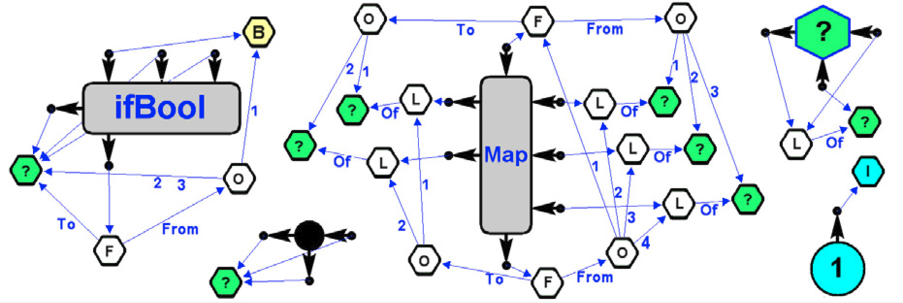
\includegraphics[width=0.505\linewidth]{images/image7.png}
\end{figure}

---------- [Const\_i]
c\_i : Int

-------------- [Const\_c]
c\_c : Char

-------------- [Const\_b]
c\_b : Bool

TODO: latexify the above, replacing sigma with rho

These typing rules can be used to deduce and prove the types of expressions. For example, the expression \mintinline{text}{|not True|} in a context $\Gamma = \{ not: Bool \rightarrow Bool \}$:

$\Gamma \vdash not : Bool \rightarrow Bool [Var]$
$\vdash True : Bool [Const\_b]$
$\Gamma \vdash not True : Bool [App]$

Despite this, the typing rules themselves aren’t an algorithm as they do not specify an order to be applied in. While only one syntax rule can apply to a subexpression, it may be unclear when to apply instantiation and generalisation. Arbitrarily applying rules does not necessarily converge to a solution, as generalisation and instantiation can both continue infinitely. For example repeatedly applying instantiation and generalisation on \mintinline{text}{|id|} with $\Gamma = \{ id: \forall a. a \rightarrow a \}$.

$\Gamma \vdash id : \forall a. a \rightarrow a [Var]$
$\Gamma \vdash id : [t0] \rightarrow [t0] [Inst] (a/[t0])$
$\Gamma \vdash id : \forall b. [b] \rightarrow [b] [Gen]$
$\Gamma \vdash id : [[t1]] \rightarrow [[t1]] [Inst] (b/[t1])$
$\Gamma \vdash id : \forall c. [[c]] \rightarrow [[c]] [Gen]$
$\Gamma \vdash id : [[[t2]]] \rightarrow [[[t2]]] [Inst] (c/[t2])$
$\dots$

The type inference algorithms W, W’ and M effectively are methods to select typing rules to determine a type for the expression, or detect the expression is incorrectly typed. While they don’t apply the typing rules directly, they are close and their respective authors prove they give equivalent results and can be implemented directly.

The algorithms are applied to abstract syntax trees, which represent the expressions in a structured way. For example, an abstract syntax tree for \mintinline{text}{|let y = (\x \rightarrow (odd x)) 3 in not y|} may be visualised as:

TODO: tree diagram of expression

The type inference algorithms are therefore tree traversal algorithms. Generally, they call themselves recursively on subtrees to process subexpressions, and then combine these results to determine a final type (the type of the root node).

Algorithm W is often seen as \textit{the} Hindley-Milner type inference algorithm. Given a context and an expression represented as an abstract syntax tree, W returns a substitution and a monotype.

The purpose of returning the type is obvious, but the purpose of the substitution is less clear. The substitution is a representation of constraints on type variables that have arisen from performing type inference on the expression. For example, given a context $\{ f: t0, not: Bool \rightarrow Bool \}$ and an expression \mintinline{text}{|not (f 3)|} we might return the type $Bool$ and the substitution $\{ t0 \mapsto Int \rightarrow Bool \}$. This substitution is important because if \mintinline{text}{|f|}\mintinline{text}{| |}or the type variable $t0$ are used elsewhere in the same expression we need to type-check those occurrences for consistency with this usage. In a wider expression such as \mintinline{text}{|[not (f 3), f True]|} the substitution from our first subexpression tells us type $t0$ is $Int \rightarrow Bool$. When examining the application of the second \mintinline{text}{|f|}, we find its type from the context which is $t0$, or equivalently now $Int \rightarrow Bool$. We can then raise a type error as we have applied it on a $Bool$.

The algorithm is set out below, for each of the five language constructs. There is a case for each type of node in the abstract syntax tree, so the rule applied at each point is deterministic and easily-chosen based on the node type. Explanations of the more complex cases are given below the algorithm.

\begin{figure}[h!]
  \centering
  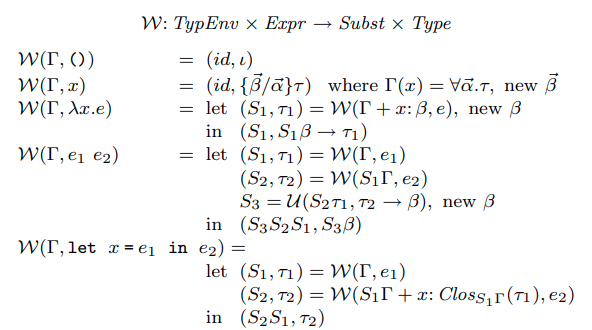
\includegraphics[width=0.987\linewidth]{images/image1.png}
\end{figure}

TODO: latexify the above (taken from Lee), replace () with constants, replace TypeEnv with Context, replace Expr with Expression, replace Subst with Substitution, replace Type with MonoType, replace Clos with generalise, add brackets around applying substitutions, add explicit combines, number the statements, replace id with \{\}, flip ordering of abs and app, replace var rule with let S\_1 = \{ a \mapsto t0, b \mapsto t1, … \}, new t0, t1, … in (id, S\_1\tau) where \Gamma(x) = \forall a \forall b … \tau

The notation $new tn$ specifies that the type variable $tn$ is new (or ‘fresh’), so its name has not been used before. Using globally unique type variables avoids reuse which may incorrectly mix constraints between different types. Most implementations use a global counter, incremented each time a new type variable is needed with names like $t0, t1, t2, \dots$.

The general structure of Algorithm W is to recursively call itself on subexpressions, until the subexpressions are simple leaf nodes. At this point, constant nodes have their assigned type and variable nodes have their type retrieved from the context. The subexpression types are passed back up, where their substitutions are either combined or fed into inferring other subexpressions, and a resultant type is returned.

Case (4app) for function application infers the types of the two subexpressions. It first infers the left one, $e\_1$, then applies the resultant substitution to the context before inferring the right subexpression, $e\_2$. This ensures constraints arising from the $e\_1$ are considered when inferring the second subexpression, so if $e\_1$ and $e\_2$ have conflicting constraints this is detected and a type error is raised. However, this does introduce a left-to-right bias where the type error is raised in the right subexpression if a conflict is found.

Given we know $e\_1$ is a function that should accept $e\_2$’s type, $\tau\_2$, we should be able to unify $\tau\_2 \rightarrow tn$ (a function accepting $\tau\_2$ and returning $tn$ i.e. anything) with the function type $\tau\_1$. We apply the substitution $S\_2$ to $\tau\_1$ when doing this to ensure no constraints have arisen in inferring $e\_2$ that would prevent this unification. Finding a unifying substitution confirms the function application is valid, and we are able to determine the return type (and thus the overall type of this expression) by applying the unifying substitution to the type variable $tn$ used as the return type. If no unifying substitution can be found, the function application is invalid (as the argument type $\tau\_2$ cannot be substituted to reach an accepted type for the function’s type $\tau\_1$) and a type error is raised. Invalid function application (4app) and undefined variables (1var) are the only possible sources of type errors from Algorithm W.

To illustrate, consider \mintinline{text}{|odd 3|} in the context $\Gamma = \{ odd: Int \rightarrow Bool \}$. We find the types of \mintinline{text}{|odd|} and \mintinline{text}{|3|} as $Int \rightarrow Bool$ and $Int$ respectively, unify $Int \rightarrow Bool$ with $Int \rightarrow t0$ to get the substitution $S\_3 = \{ t0 \mapsto Bool \}$ and return the overall type $S\_3(tn) = \{ t0 \mapsto Bool \}t0 = Bool$.

Also consider \mintinline{text}{|odd x|} in the context $\Gamma = \{ odd: Int \rightarrow Bool, x: t0 \}$. Here we find the types of \mintinline{text}{|odd|} and \mintinline{text}{|x|} as $Int \rightarrow Bool$ and $t0$ respectively, unify $Int \rightarrow Bool$ with $t0 \rightarrow t1$ to get the substitution $S\_3 = \{ t0 \mapsto Int, t1 \mapsto Bool \}$ and return the overall type $S\_3(tn) = \{ t0 \mapsto Int, t1 \mapsto Bool \}t1 = Bool$. In this we also return the substitution $\{ t0: Int, t1: Bool \}$, constraining the external type $t0$ to an $Int$. Given we created $t1$ as a new type variable, it won’t be found elsewhere so does not need to be considered in other expressions so the substitution $\{ t0 \mapsto Int \}$ could equivalently have been returned.

Case (3abs) for function abstraction first infers the type of the function body expression, $e$, by calling W recursively. It passes the current context with an additional binding for the function parameter $x$, assigned to a new type variable with no constraints. This subcall to W for the function body returns the substitution $S\_1$ and type $\tau\_1$. Finally, the substitution $S\_1$ and type $S\_1(tn \rightarrow \tau\_1)$ is returned as the final result for the function abstraction. The type arises from the fact that the function abstraction takes the parameter with the new type $tn$ and returns the type of the body, $\tau\_1$. We apply the substitution $S\_1$ to it to reflect any constraints on the function parameter picked up in the function body.

For an example examine calling W on \mintinline{text}{|\x \rightarrow odd x|} with $\Gamma = \{ odd: Int \rightarrow Bool \}$. The subcall to W calls $W(\Gamma + x: t0, odd x)$ which returns $(S\_1, \tau\_1) = (\{ t0: Int \}, Bool)$. Then $(S\_1, S\_1(tn \rightarrow \tau\_1)) = (\{ t0 \mapsto Int \}, \{ t0 \mapsto Int \}(t0 \rightarrow Bool)) = (\{ t0 \mapsto Int \}, Int \rightarrow Bool)$ is returned as the result.

Case (5let) for let statements first infers the type $\tau\_1$ of the parameter definition, $e\_1$. The parameter type $\tau\_1$ is then generalised with respect to the context to allow for polymorphism as per HM’s type system, before being added to the context as a binding and used to infer the let body $e\_2$. The substitutions $S\_1$ and $S\_2$ are then combined to collect the constraints, and are returned with the let body’s type $\tau\_2$.

Algorithm W’ is a slightly altered variant of Algorithm W, only changing rule (4app) for function application to avoid left-to-right bias.

\begin{figure}[h!]
  \centering
  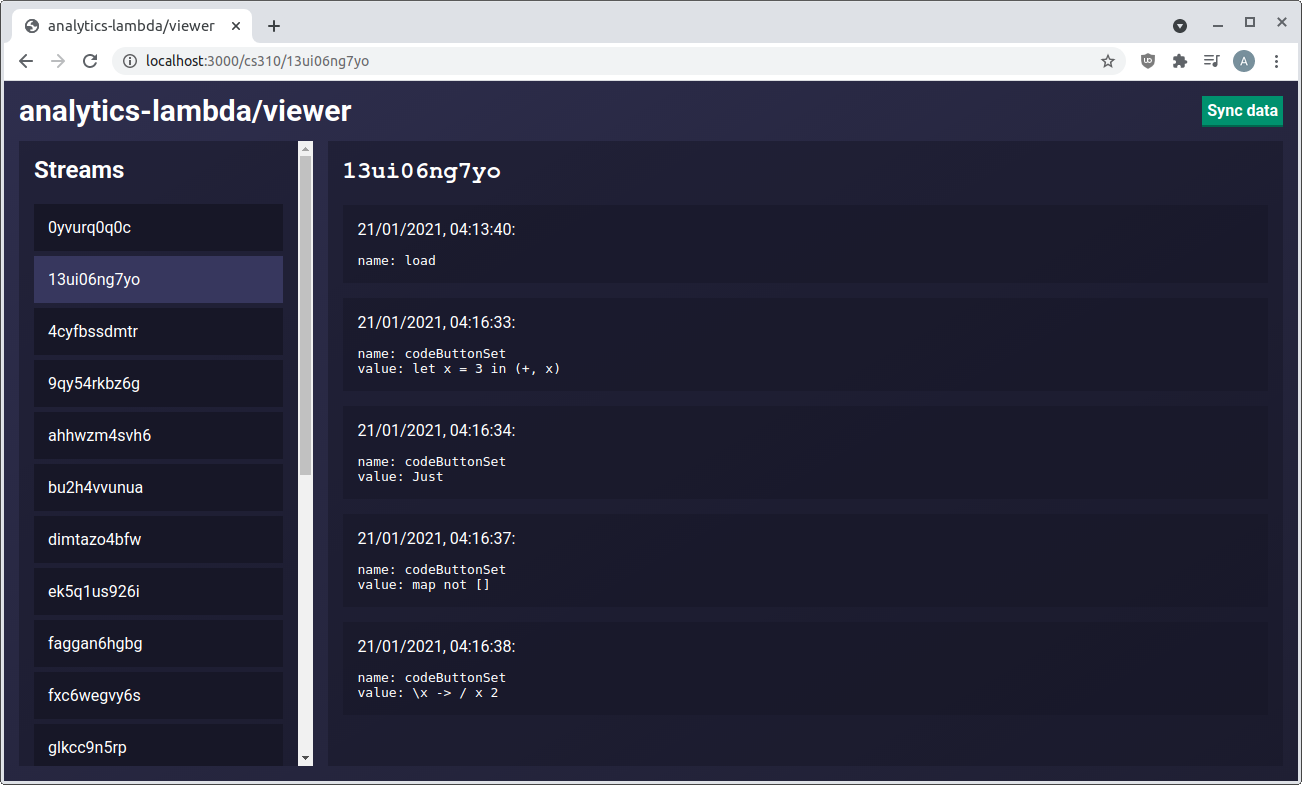
\includegraphics[width=0.782\linewidth]{images/image14.png}
\end{figure}

TODO: write out algorithm in Lee format for W’, 1-index, replace S’ with S\_3, V with S\_4

Algorithm W’ performs substitution unification, introduced in the same paper as W’. Like type unification, substitution unification attempts to find a unifying substitution to unify two values. Unlike type unification, substitution unification attempts to make two substitutions, not types, equal. It returns a unifying substitution, which when combined with either substitution gives the same result, i.e. $combine(unify(S\_1, S\_2), S\_1) = combine(unify(S\_1, S\_2), S\_2)$. Both type and substitution unification is commutative and associative, and may fail if no such substitution exists.

If substitutions share no type variables, finding a unifying substitution can be done by simply combining the substitutions. For example, $unify(\{ t0 \mapsto Int \}, \{ t1 \mapsto Bool \}) = combine(\{ t0 \mapsto Int \}, \{ t1 \mapsto Bool \}) = \{ t0 \mapsto Int, t1 \mapsto Bool \}$.

However, substitution unification generally is different to substitution combination. Combination only simulates the effect of applying consecutive substitutions, so is not concerned with unifying substitution types or maintaining constraints. For example, given $S\_1 = \{ t0 \mapsto t1 \rightarrow Bool \}$ and $S\_2 = \{ t0 \mapsto Int \rightarrow t2 \}$, then $S\_3 = unify(S\_1, S\_2) = \{ t1 \mapsto Int, t2 \mapsto Bool \}$, which is not the same as combining the substitutions. Note the resultant unifying substitution may have a non-empty domain disjoint from both the given substitutions, as in this example. We can see that $combine(S\_3, S\_1) = combine(S\_3, S\_2) = \{ t0 \mapsto Int \rightarrow Bool, t1 \mapsto Int, t2 \mapsto Bool \}$.

Having defined substitution unification, case (4app) in W’ is fairly straightforward. It independently infers the two subexpressions $e\_1$ and $e\_2$, rather than applying $e\_1$’s substitution $S\_1$ to the context before inferring $e\_2$ as in W. The substitutions are then unified and then applied to both subexpression types, ensuring all constraints are applied to both types. The function type and the argument to new type can then be unified in the same way as W.

Algorithm M is a top-down approach to type inference. Implemented as part of an early ML compiler by~\cite{ref32}, it was known as a ‘folklore’ algorithm until~\cite{ref33} formalised it as in the figure below.

Given a context, expression and type it returns a substitution. When compared to W’s signature, this effectively moves the type from the output of W to the input of M. The input type now represents an expected type for the expression, to be checked and then refined by returning a substitution. Types are refined as they progress down the tree (hence top-down), and if they are found to be incompatible at any point a type error is raised. In some cases this can lead to more specific error messages as type errors are generally raised lower down the tree, rather than at potentially more complex function application expressions as in W. More specific error messages are more useful for developers to identify where the bugs are in their programs.

M is initially started at the root node with a new type, i.e. $M(\Gamma, e, tn), new tn$, and the final type can be determined by applying the returned substitution to $tn$. In this way both type inference algorithms can be wrapped to have the signature $Context \times Expression \rightarrow Type$ which would be naturally expected from type inference algorithms.

\begin{figure}[h!]
  \centering
  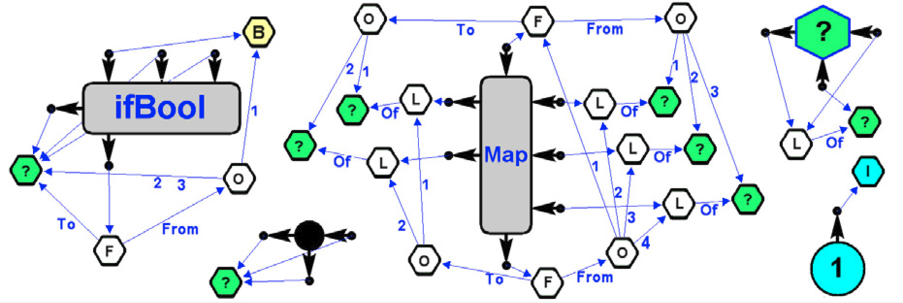
\includegraphics[width=1.000\linewidth]{images/image4.png}
\end{figure}

TODO: latexify the above (taken from Lee), make replacements as per W alg, replace rho with tau\_e

M has some similarities to W, however where W applies unification in function application, M instead pushes this down the tree and performs unification in the leaf nodes and function abstraction.

In rules (1con) and (2var) for constant and variable expressions, we are given an expected type $\tau\_e$ and are verifying it can unify with the literal constant’s type or the type from the context respectively. Unifying in this way returns the type in the substitution, for example $M(\{\}, 3, t0) = unify(Int, t0) = \{ t0: Int \}$ and $M(\{ odd: Int \rightarrow Bool \}, odd, t0 \rightarrow t1) = unify(Int \rightarrow Bool, t0 \rightarrow t1) = \{ t0: Int, t1: Bool \}$, which is passed back up the tree.

Rule (4app) shows function application in M has no unification step. Instead, M is simply called recursively for each expression. The first expression, $e\_1$, is expected to be a function taking a new type variable $tn$ and returning the expected type $\tau\_e$ for the overall application. The second expression should have the argument type for the function, $tn$, after applying substitution $S\_1$ to collect type constraints.

For example, consider \mintinline{text}{|odd 3|} in the context $\Gamma = \{ odd: Int \rightarrow Bool \}$ with expected type $t0$. We call M with the expected type $t1 \rightarrow t0$ on \mintinline{text}{|odd|} to get the substitution $S\_1 = \{ t1: Int, t0: Bool \}$. We then call M with the expected type $S\_1(t1) = Int$ on \mintinline{text}{|3|}, which is validated and returns an empty substitution $S\_2 = \{\}$. Finally, we return the combined substitution $\{ t1: Int, t0: Bool \}$.

In rule (3abs) for function abstraction, we verify the expected type unifies with a new function type. This gives a substitution mapping the variables $t1$ and $t2$ to the expected function types, if any. This is applied to the context, along with adding the parameter $x$’s type as $t1$. We then use M to infer the type of the function body, expecting it to have the unified return type $t2$. We return the combined substitution from both parts.

For an example we look at applying M on \mintinline{text}{|\x \rightarrow odd x|} with $\Gamma = \{ odd: Int \rightarrow Bool \}$ and expected type $t0$. We first unify $t0$ with the new type $t1 \rightarrow t2$, resulting in $S\_1 = \{ t0: t1 \rightarrow t2 \}$. We then make the recursive call to M with the function body \mintinline{text}{|odd x|}, context $\{ odd: Int \rightarrow Bool, x: t1 \}$ and expected type $t2$. This results in the substitution $S\_2 = \{ t1: Int, t2: Bool \}$, which we combine with $S\_1$ to get $combine(S\_2, S\_1) = \{ t0: Int \rightarrow Bool, t1: Int, t2: Bool \}$. As in W’s function application, the new type variables will be unused outside of this expression so we can equivalently exclude $t1$ and $t2$ from the substitution.

Finally, let expressions infer the type of their parameter $e\_1$ with a new type, then infer the type of their body $e\_2$ expecting it to have the overall expected type $\tau\_e$. Similarly to function abstraction, the substitution from the parameter is passed when inferring the body, and combined with the body’s substitution to give an overall result.

These type inference algorithms do have limitations. They all sometimes produce poor type error messages; Algorithm W often detects errors late, highlighting too large of a subexpression to be useful and Algorithm M often detects too specific of a term without context as to what original definition it violates. Algorithm W has the left-to-right bias which Algorithm W’ attempts to correct for, however this can sometimes exacerbate the problem with highlighting large subexpressions. Poor error messages make it difficult for the programmer to understand how to fix the problem.

To improve error messaging, hybrid or constraint-based algorithms along with heuristics are often used in practice to provide more informative error messages. Reducing the size of the amount inferred at once can help make errors more precise. For example, Apple’s Swift uses a bi-directional type inference algorithm on single statements \citep{ref34}.

Additionally, despite not being required in all languages, explicit type annotations are often used to help identify errors earlier at locations which are easier to interpret \citep{ref35}. This is especially common for function definitions or program entry points. This also effectively splits up the program into smaller parts which can be inferred against separately, improving performance and making type errors more precise. In some cases, type inference algorithms struggle with (directly or indirectly) recursively defined functions and type annotations can help define these types. Finally, changing a rigidly-typed interface also highlights potential breaking changes to libraries or helper functions. In this way type annotations act as documentation to future programmers using the code. Manually specified, more specific types may be an improvement over automatically inferred types as sometimes the most general type as worked out by a type inference algorithm may not clearly convey the intent of the programmer.

TODO: (maybe?) Add a section on type errors. Resources:

\underline{\href{https://www.researchgate.net/profile/Jurriaan\_Hage/publication/221241370\_Scripting\_the\_Type\_Inference\_Process/links/02e7e51a37f9233c65000000.pdf}{https://www.researchgate.net/profile/Jurriaan\_Hage/publication/221241370\_Scripting\_the\_Type\_Inference\_Process/links/02e7e51a37f9233c65000000.pdf}}
Improving type error messages

\underline{\href{https://dspace.library.uu.nl/bitstream/handle/1874/7297/full.pdf?sequence=8}{https://dspace.library.uu.nl/bitstream/handle/1874/7297/full.pdf?sequence=8}}
Top quality type error messages

\underline{\href{https://manu.sridharan.net/files/mycroft-preprint.pdf}{https://manu.sridharan.net/files/mycroft-preprint.pdf}}
A Practical Framework for Type Inference Error Explanation

\underline{\href{http://citeseerx.ist.psu.edu/viewdoc/download?doi=10.1.1.110.5050\&rep=rep1\&type=pdf}{http://citeseerx.ist.psu.edu/viewdoc/download?doi=10.1.1.110.5050\&rep=rep1\&type=pdf}}
PhD thesis which talks about hindley milner and type inference errors a lot
\section{Design}\label{id:h.7ggvdxb04tzm}
The design of the teaching tool is split into two parts, working backwards from the end product in mind: designing the user interface and experience, and designing the architecture to support that.
\subsection{User interface and experience}\label{id:h.dr046u473e01}
Before designing the new teaching tool, we explore the existing available resources to see what works well, and what is missing. The current resources for learning about type inference can be generally categorised into three categories: programming language documentation, formal resources and informal resources. These resources were found by examining the pages returned by the first 5 pages of Google search on the query ‘type inference’. The following is a summary of what was found from reading these resources with the aim of determining their strengths and weaknesses.

Programming language documentation are pages written to explain how type inference works in a specific language, as part of that language’s official documentation. For example, TypeScript, Java and Golang all have official websites where they discuss how type inference works in their language.

Formal resources include university lecture notes, papers on type inference or encyclopedias. The first two are often in PDF format or on archiving websites. Wikipedia and WikiWikiWeb are examples of the latter (while encyclopedias summarise the subject they are generally written formally, with a lot of mathematical notation hence fall in this category).

Informal resources include personal blog posts and online talk recordings. These are generally written by developers interested in programming language design or compiler development.

Each category of resource covers different aspects of type inference.

Formal resources generally cover the most generic and widely-applicable concepts in a succinct manner. They usually present type inference in the context of the Hindley-Milner system, or a related functional language such as ML or OCaml. Formal resources usually detail how type inference algorithms (usually algorithm W) go about determining types, and the specific rules of the type system they operate in. It is rare for them to discuss how type errors are treated or give examples of error cases.

Programming language documentation covers type inference in the context of a specific language, with all results inspected giving code examples along with text explaining what the code is doing. Generally this documentation explains the features of type inference present in the language, rather than the wider concepts, although does so in a directly-applicable way. Some languages also explain language-specific concepts in detail, such as how type inference works with Java’s generics or TypeScript’s functions. They are also tailored to how languages are used, with Java’s documentation exploring how type inference is applied in object-oriented programming and TypeScript giving examples of type inference with web APIs. They often do not discuss how the type inference algorithms determine the types, but rather just what the types are and roughly the rules of the type system. However, they do usually give sufficient examples to understand the type system, with languages such as TypeScript, Java and Scala including error cases and explanations on how to fix the type errors. These error examples are particularly helpful as they show how a programmer might go about debugging and fixing type errors found in their program.

Informal resources generally discusses personal reflections on what the author has learnt about type inference or they heavily focus on type inference’s application within a specific language the author is familiar with. These are generally the least widely-applicable, and often only cover a small part of a single programming language, however do so in great detail and often giving practical advice about work related to their subject matter.

Resources also differ in accessibility: how easy it is for a user to read, understand and apply their content.

Programming language documentation and informal resources both are generally aimed at a more clearly targeted audience, usually programmers using a specific language. They are written in simpler language and use significantly less notation than formal resources which makes them easier reading. Their use of examples makes concepts clearer, and many of them have a level of interactivity which allows readers to try things for themselves, allowing readers to test their own knowledge or verify something that isn’t clear to them from the documentation alone. For example TypeScript’s documentation allows users to hover over code samples to inspect the types as well as open it up in an online coding environment, while Golang and Rust’s respective documentation sites have example programs which users are encouraged to edit and run online. Blog posts often have code snippets or GitHub gists for users to run, and in talks presenters may give live coding demos, which serve similar purposes.

\begin{figure}[h!]
  \centering
  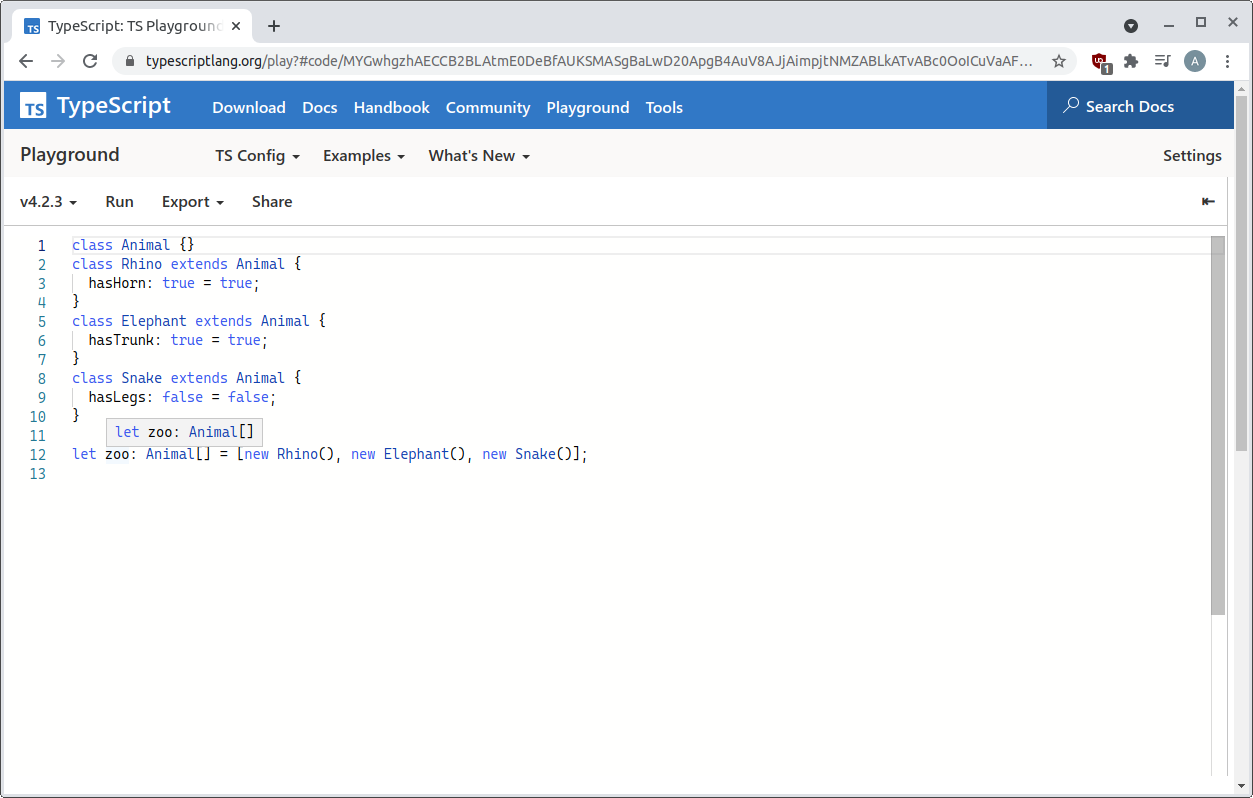
\includegraphics[width=1.000\linewidth]{images/image5.png}
  \caption{The TypeScript playground, with an example opened from the Type Inferece documentation showing how JavaScript classes can work in TypeScript.}
\end{figure}

\begin{figure}[h!]
  \centering
  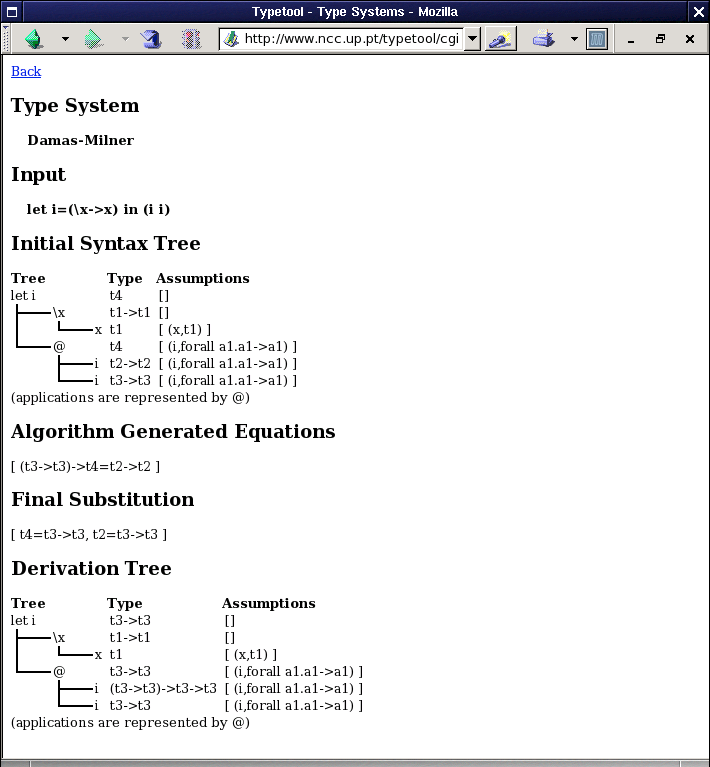
\includegraphics[width=1.000\linewidth]{images/image2.png}
  \caption{Golang's limited type inference is explained in 'A Tour of Go', with an example program the user is prompted to edit and run.}
\end{figure}

\begin{figure}[h!]
  \centering
  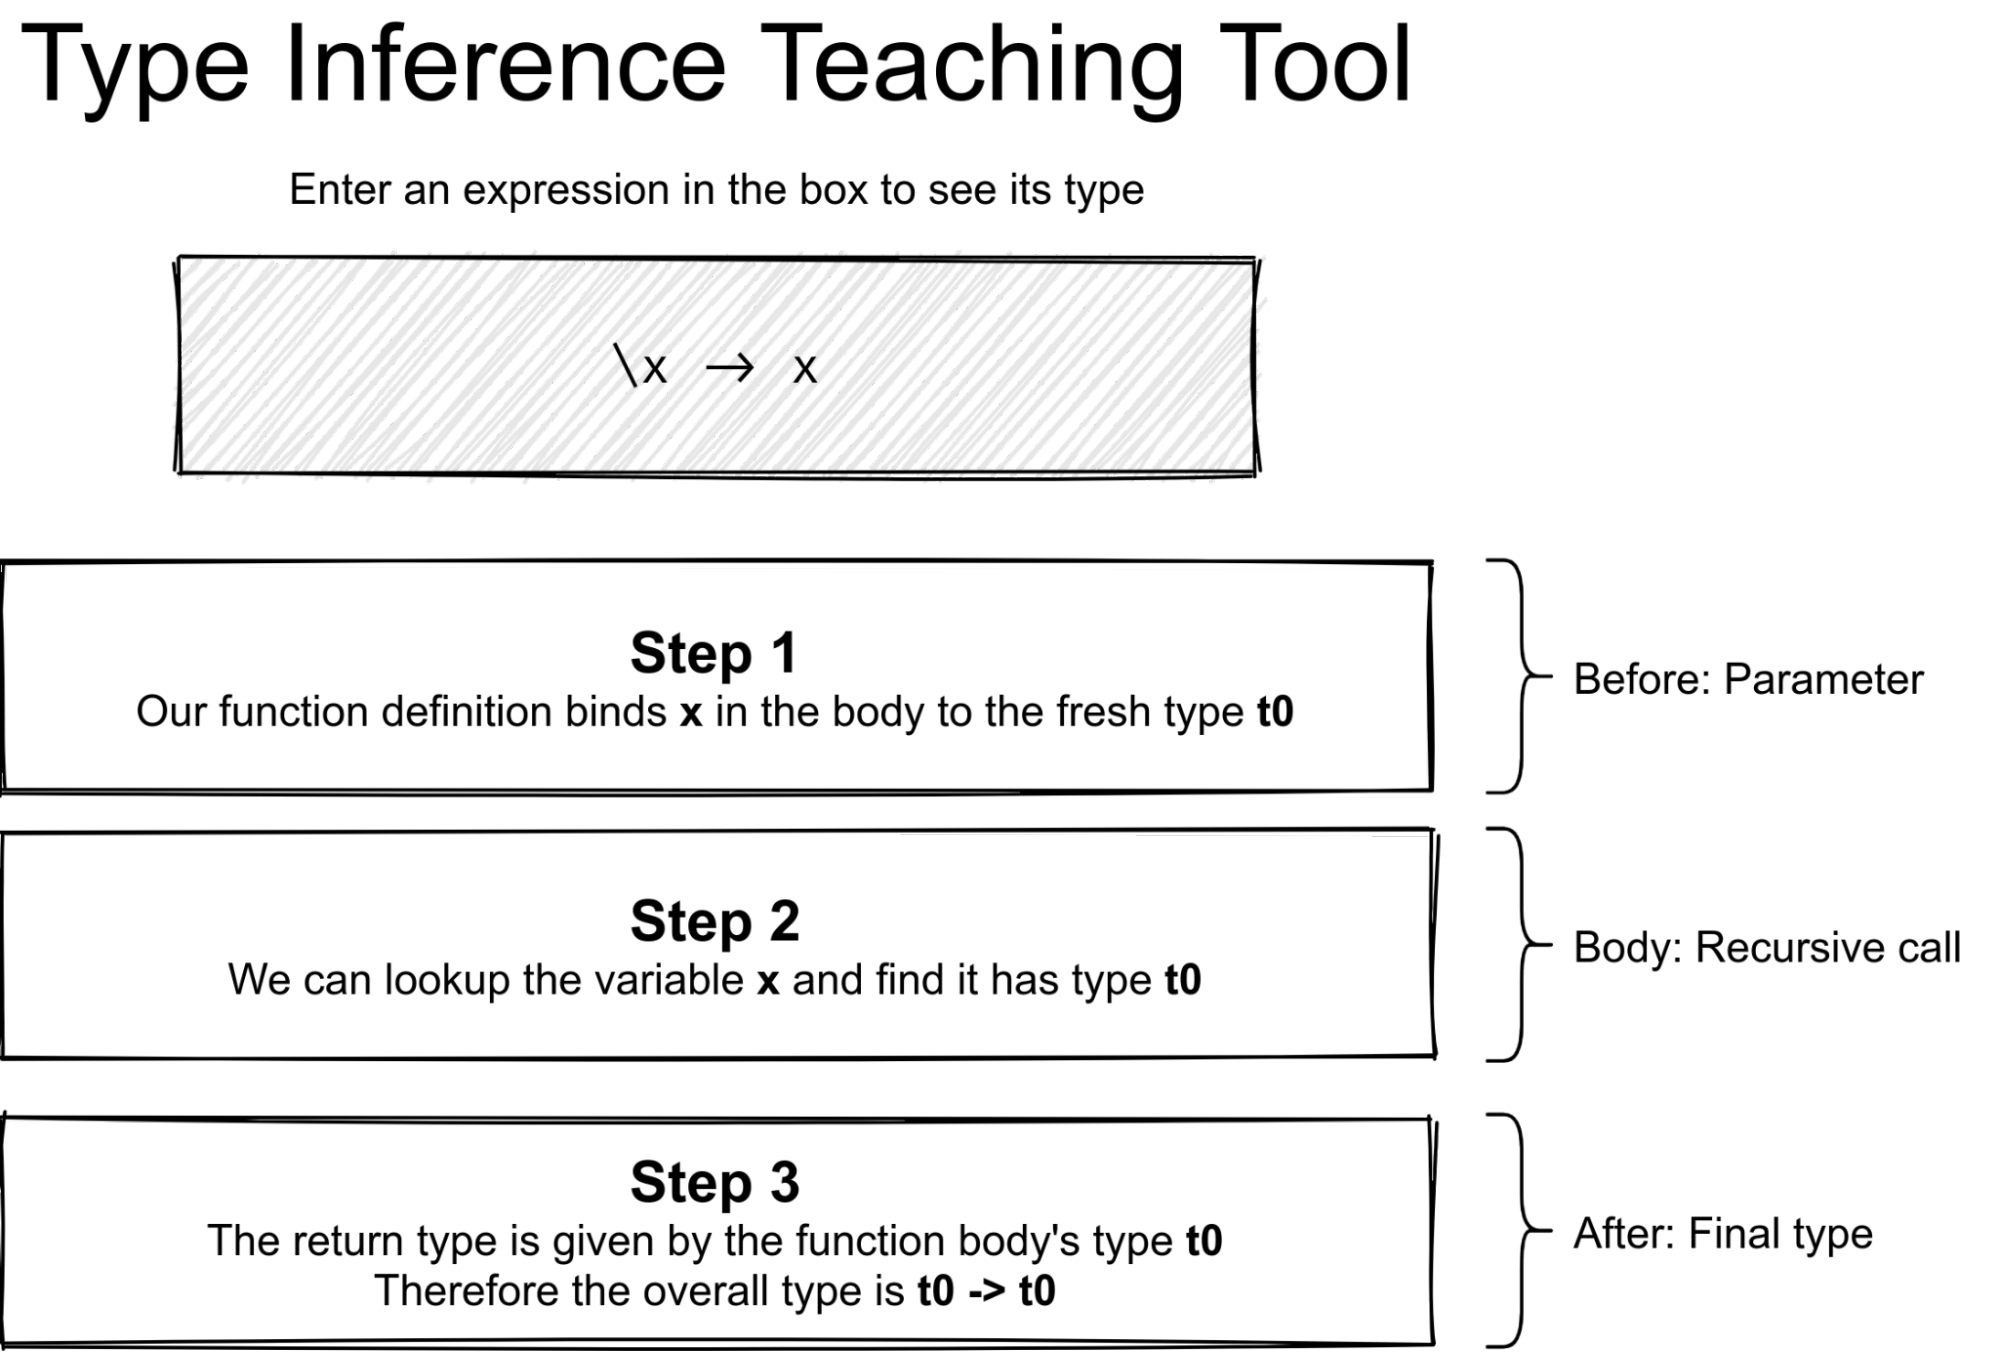
\includegraphics[width=1.000\linewidth]{images/image15.png}
  \caption{Rust's page on type inference is short, but has a well-commented and insightful example that can be run and edited inline in the browser.}
\end{figure}

Formal resources are usually aimed at a more mathematically-inclined audience, with less specific focus on any language or technology. It often uses mathematical terms and notation to convey ideas, which some readers may find difficult to understand. In particular, papers are often written in a very precise and succinct way with few examples, which can make them hard to interpret. This is likely due to the length constraints put in place by academic journals which incentives authors to cut more detailed explanations and examples from their work. Few papers and lecture notes would be immediately accessible to the general computer scientist, as papers often assume the reader has a strong grounding in the field already and lecture nodes are meant to be read in order, expecting the reader to have read the previous 20 lectures worth of notes. However, they do usually give clear and useful references for background and further reading which is useful for in-depth research on the topic, if not for an introduction. The implementation of a type inference algorithm and how it is applied to a specific language is rarely discussed. Where it is discussed the only languages used were Haskell, ML and OCaml. According to the StackOverflow Developers Survey\footnote{\underline{\href{https://insights.stackoverflow.com/survey/2020\#technology-programming-scripting-and-markup-languages}{https://insights.stackoverflow.com/survey/2020}}} Haskell is used by 1.8\% of professional developers, while ML and OCaml are very rarely used in practice. These examples may therefore be of limited use to explain to developers how type inference is used in languages they are familiar with.



Finally, the different nature of resources means some are harder to correct or update with new information.

Informal resources generally seem to have the most errors, likely because it has little review process and may be written by anyone. Sometimes through comments other readers can provide corrections or clarifications, but these are not always incorporated into the material. However, commenting is not always available and also given the specific nature of some content few people are likely to view and suggest corrections to the content. Additionally, as informal resources are usually published as one-off talks or blog posts, it is rare for the document to be maintained and kept updated which can lead to inaccuracies if the underlying technology they are discussing has made breaking changes to its implementation.

Programming language documentation on type inference is generally accurate and well maintained. It is kept up to date with changes to the language, as usually there is a requirement to keep documentation updated in programming language projects. Additionally, almost all programming languages are open source and welcome external contributions to their documentation so readers are able to suggest improvements or raise issues about inaccuracies. Generally there is a review process, often requiring a maintainer of the programming language to approve the changes before edits are made.

Formal resources generally have few errors. For academic papers, this is likely a result of the peer-review process. Lecture notes are generally written by academics with relevant qualifications and educational backgrounds, who are likely to be knowledgeable on the subject. However, academic papers and lecture notes are unlikely to be updated, which means any inaccuracies in them are harder to correct. Exploring the literature we find there are some papers on type inference with errors which make understanding them fully more difficult. Finally, online encyclopedias can be reviewed and edited by many people, whose combined expertise generally results in accurate articles although they are prone to errors being introduced by even just a single contributor if they lack a review process. Luckily, except for errors, formal resources are unlikely to become outdated with time as much as informal resources. This is because formal resources focus on the more general underlying concepts over discussion on a specific implementation.

This exploration into existing teaching resources is summarised in the table:



\begin{adjustbox}{center}\begin{tabular}{ |l|l|l|l| }
  \hline
   & \textbf{Content} & \textbf{Accessibility} & \textbf{Correctness} \\
  \hline
  \textbf{Programming language documentation} & Explains how type inference is applied in the context of a specific programming language including error cases. & Written in plain language with code samples and often interactive environments. & Few errors, and generally well-maintained. Content may change as rules of the language do. \\
  \hline
  \textbf{Formal resources} & Explains how type inference works at a general level. & Often uses complex or mathematical notation and requires significant background reading, and is sometimes too brief at the expense of clarity. & Few errors, although errors that do exist may persist given some resources can be hard to update. Generally relevant for a long time. \\
  \hline
  \textbf{Informal resources} & Contains practical tips, however usually very specific and irrelevant to many programmers. & Written in plain language with many code samples. & Inaccuracies are common, and often go undetected or unresolved. Can become outdated quickly. \\
  \hline
\end{tabular}\end{adjustbox}\\

TODO: (maybe?) discuss my exploration of existing teaching tools (wolframalpha, khanacademy, cymath, microsoft math, css diner)

This research into existing resources identifies strengths and weaknesses of different approaches. Given that this project is a one-off piece of work and the end product may not be maintained indefinitely, research into the content, correctness and longevity of resources suggests that the focus should be on the more general type inference concepts rather than specific programming language features. The tool should support error cases, not just correctly-typed expressions. It should be reviewed by my project supervisor tested with users to identify errors that can be resolved before project completion. To aid accessibility text should be written in plain language, the tool should offer several insightful examples and the output should avoid overuse of complex notation.

As a tool that displays the output of type inference algorithms, to further determine the user interface for the output of the tool the presentation of type inference proofs is examined. My supervisor initially gave some examples of worked proofs for type inference, which also matched the format of proofs found in papers and in online resources. These proofs are broken down into steps, which each look at a particular subexpression and apply a certain typing rule. Depending on the type of proof (whether it is based purely on the typing rules or is more procedural and similar to an algorithm), this may also result in explicit unification resulting in a substitution to be applied.

Based on this, the tool is designed to show the result of type inference on an expression broken into steps. Given that the tool will be automated, the steps must be generated based on some deterministic procedure and so the steps will correspond to those of the type inference algorithms. This means the steps will need to show the unification operations performed and the resultant substitutions to fully explain how the types are being inferred.

A basic UI mockup is shown below that takes an input expression and displays the inference algorithm steps beneath it. While simple, it is fundamentally similar to the final design of the application. It was also at this design that it was decided to show the type derivation feedback instantly on the same page, based on the limitations of previous related work and the strength of interactive playgrounds in programming language documentation. On top of this design, the final application adds a choice of algorithms, several samples to choose from and a display of the final type. In addition, the final application shows and explains the steps of the type inference algorithm when type errors are present.

{\centering \begin{figure}[h!]
  \centering
  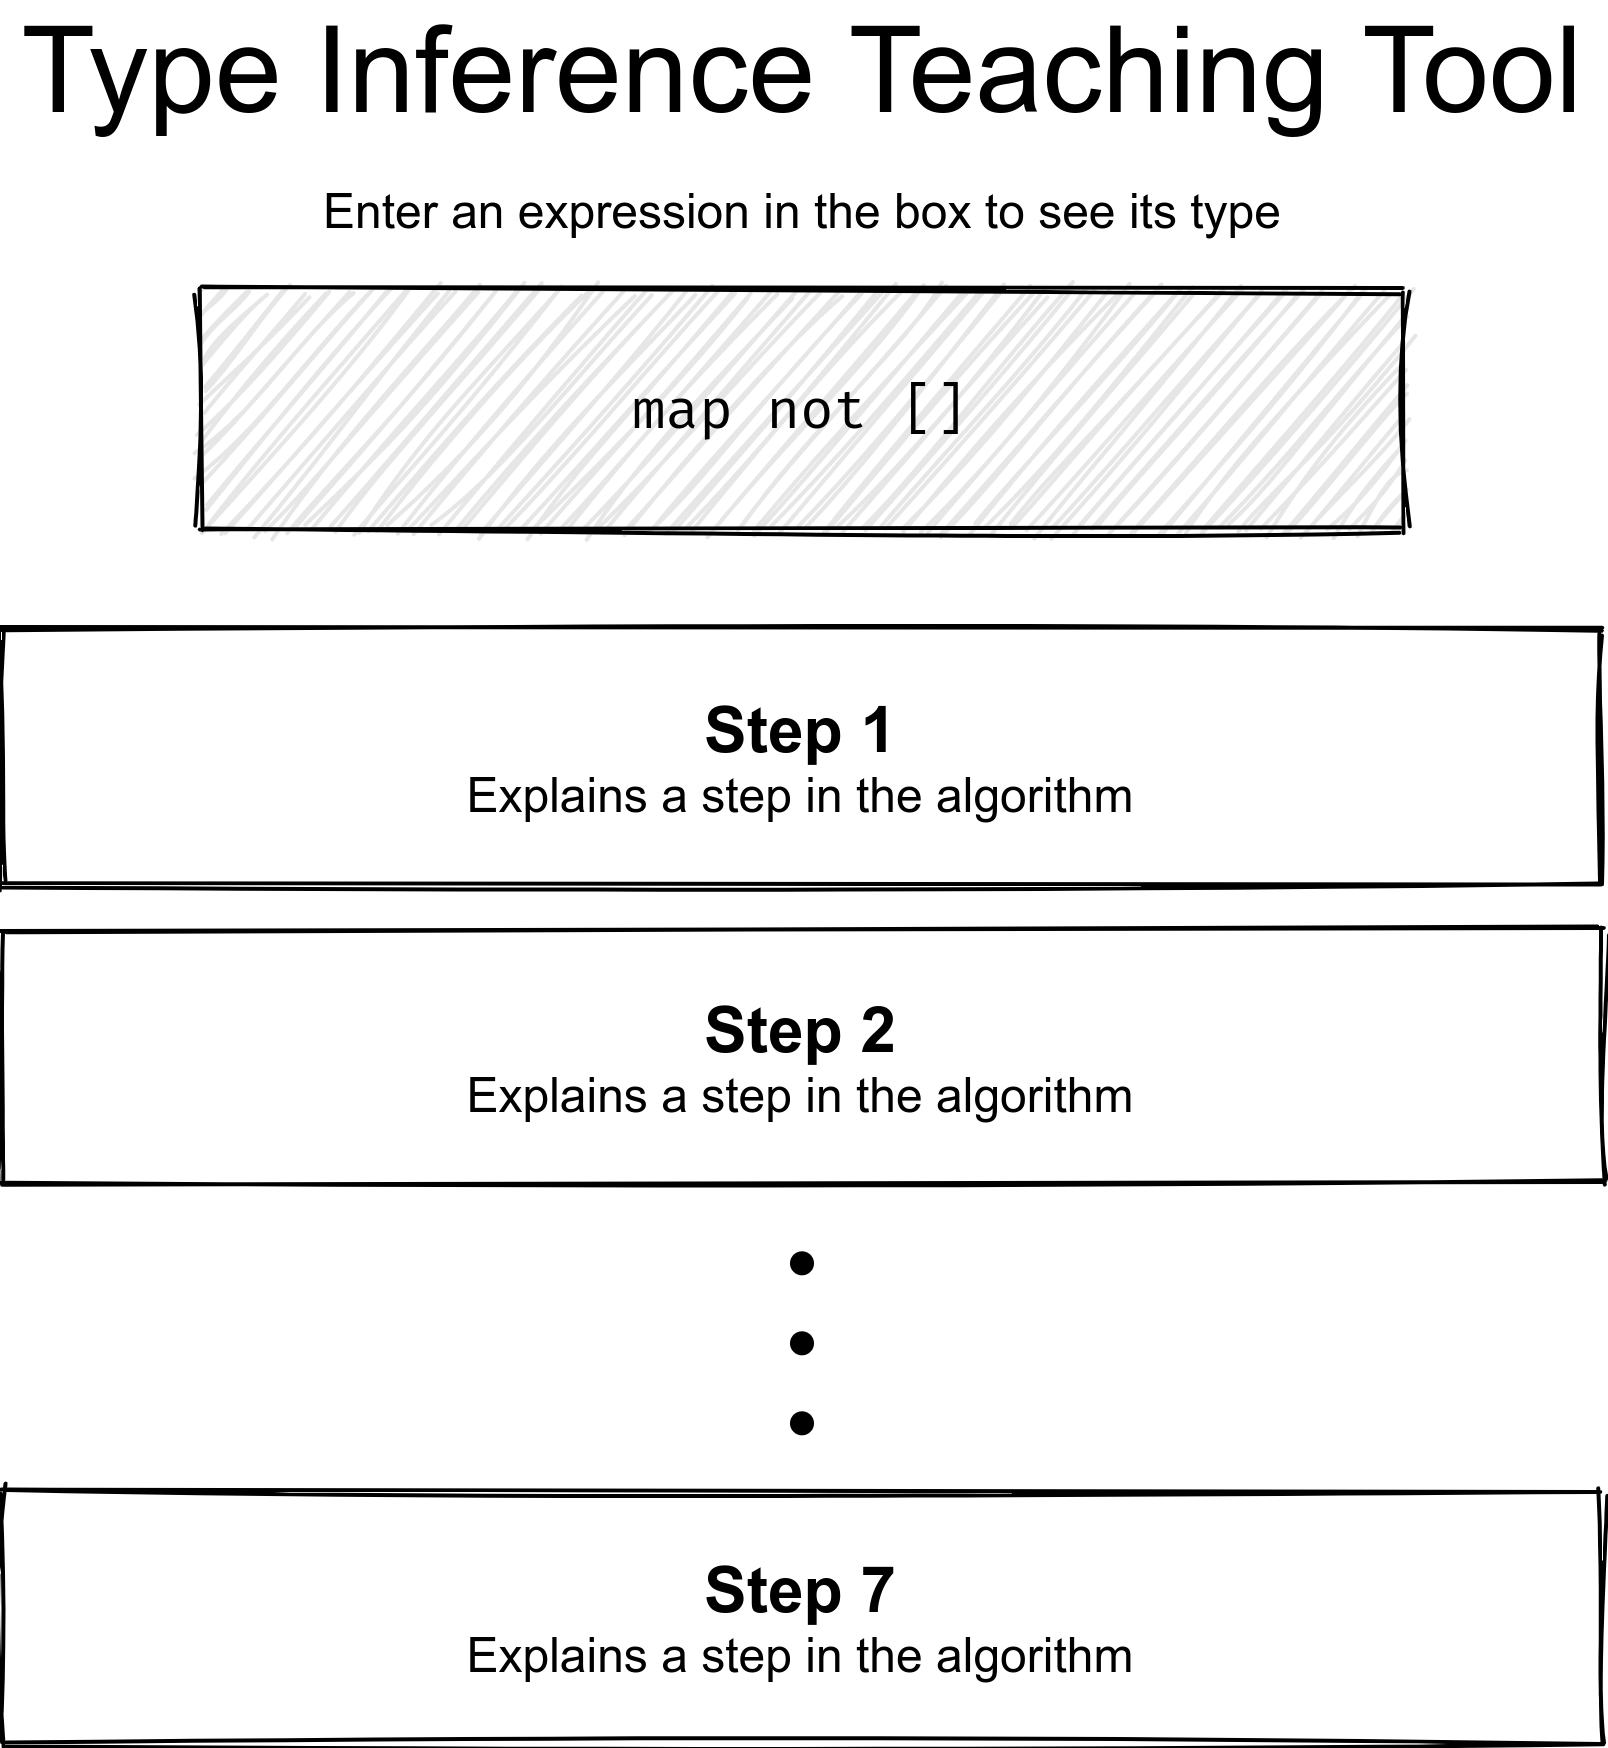
\includegraphics[width=0.756\linewidth]{images/image13.png}
  \caption{Recreation of an initial sketch of the UI for the teaching tool.}
\end{figure} \par}

A step in the UI generally corresponds to a rule of the type inference algorithm. As the type inference algorithms are recursive, some rules may call the type inference algorithms again on a subexpression. In these cases it may be necessary to split rules of the type inference algorithm up into two parts, before and after a recursive call. This helps ensure the ordering of the steps makes logical sense.

For example, this happens with function abstraction in algorithm W: the before step shows assigning a new type variable as the parameter’s type, steps between show the results of the recursive call to the body, while the after step details the final type of the function abstraction expression.

{\centering \begin{figure}[h!]
  \centering
  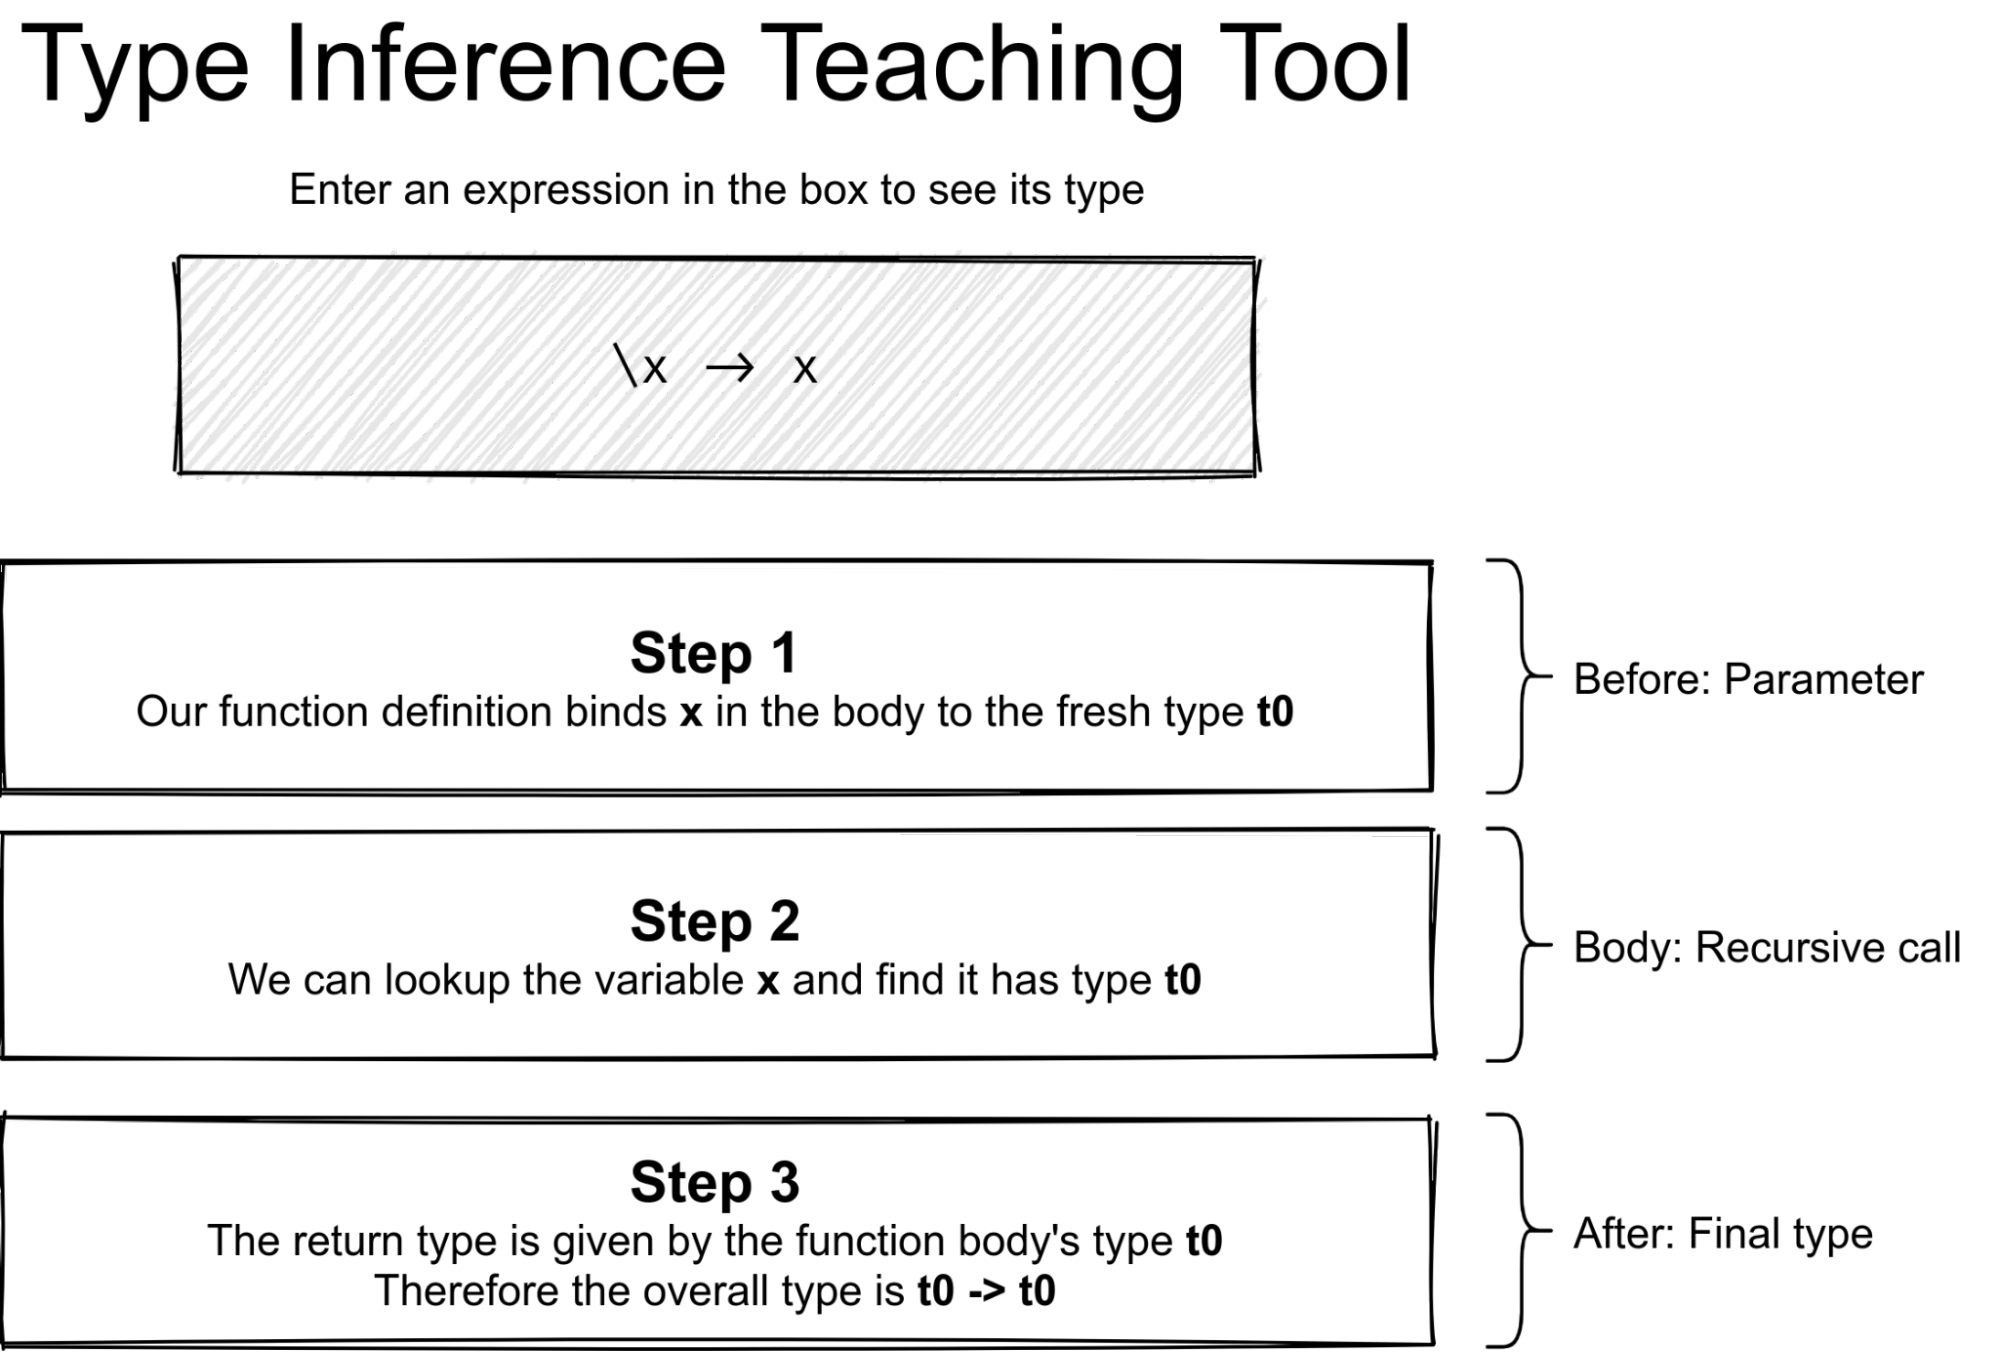
\includegraphics[width=0.945\linewidth]{images/image9.png}
  \caption{Function abstraction in algorithm W requires two UI steps to represent one rule of the algorithm}
\end{figure} \par}

In addition to the rule steps, algorithm M requires an extra beginning and end step. These are required as algorithm M requires an input type and does not return a type respectively. The first step is to create an initial new type $t0$ for the root node, and the final step is added to apply the final substitution to type $t0$ (effectively the value of $t0$ from the substitution).

{\centering \begin{figure}[h!]
  \centering
  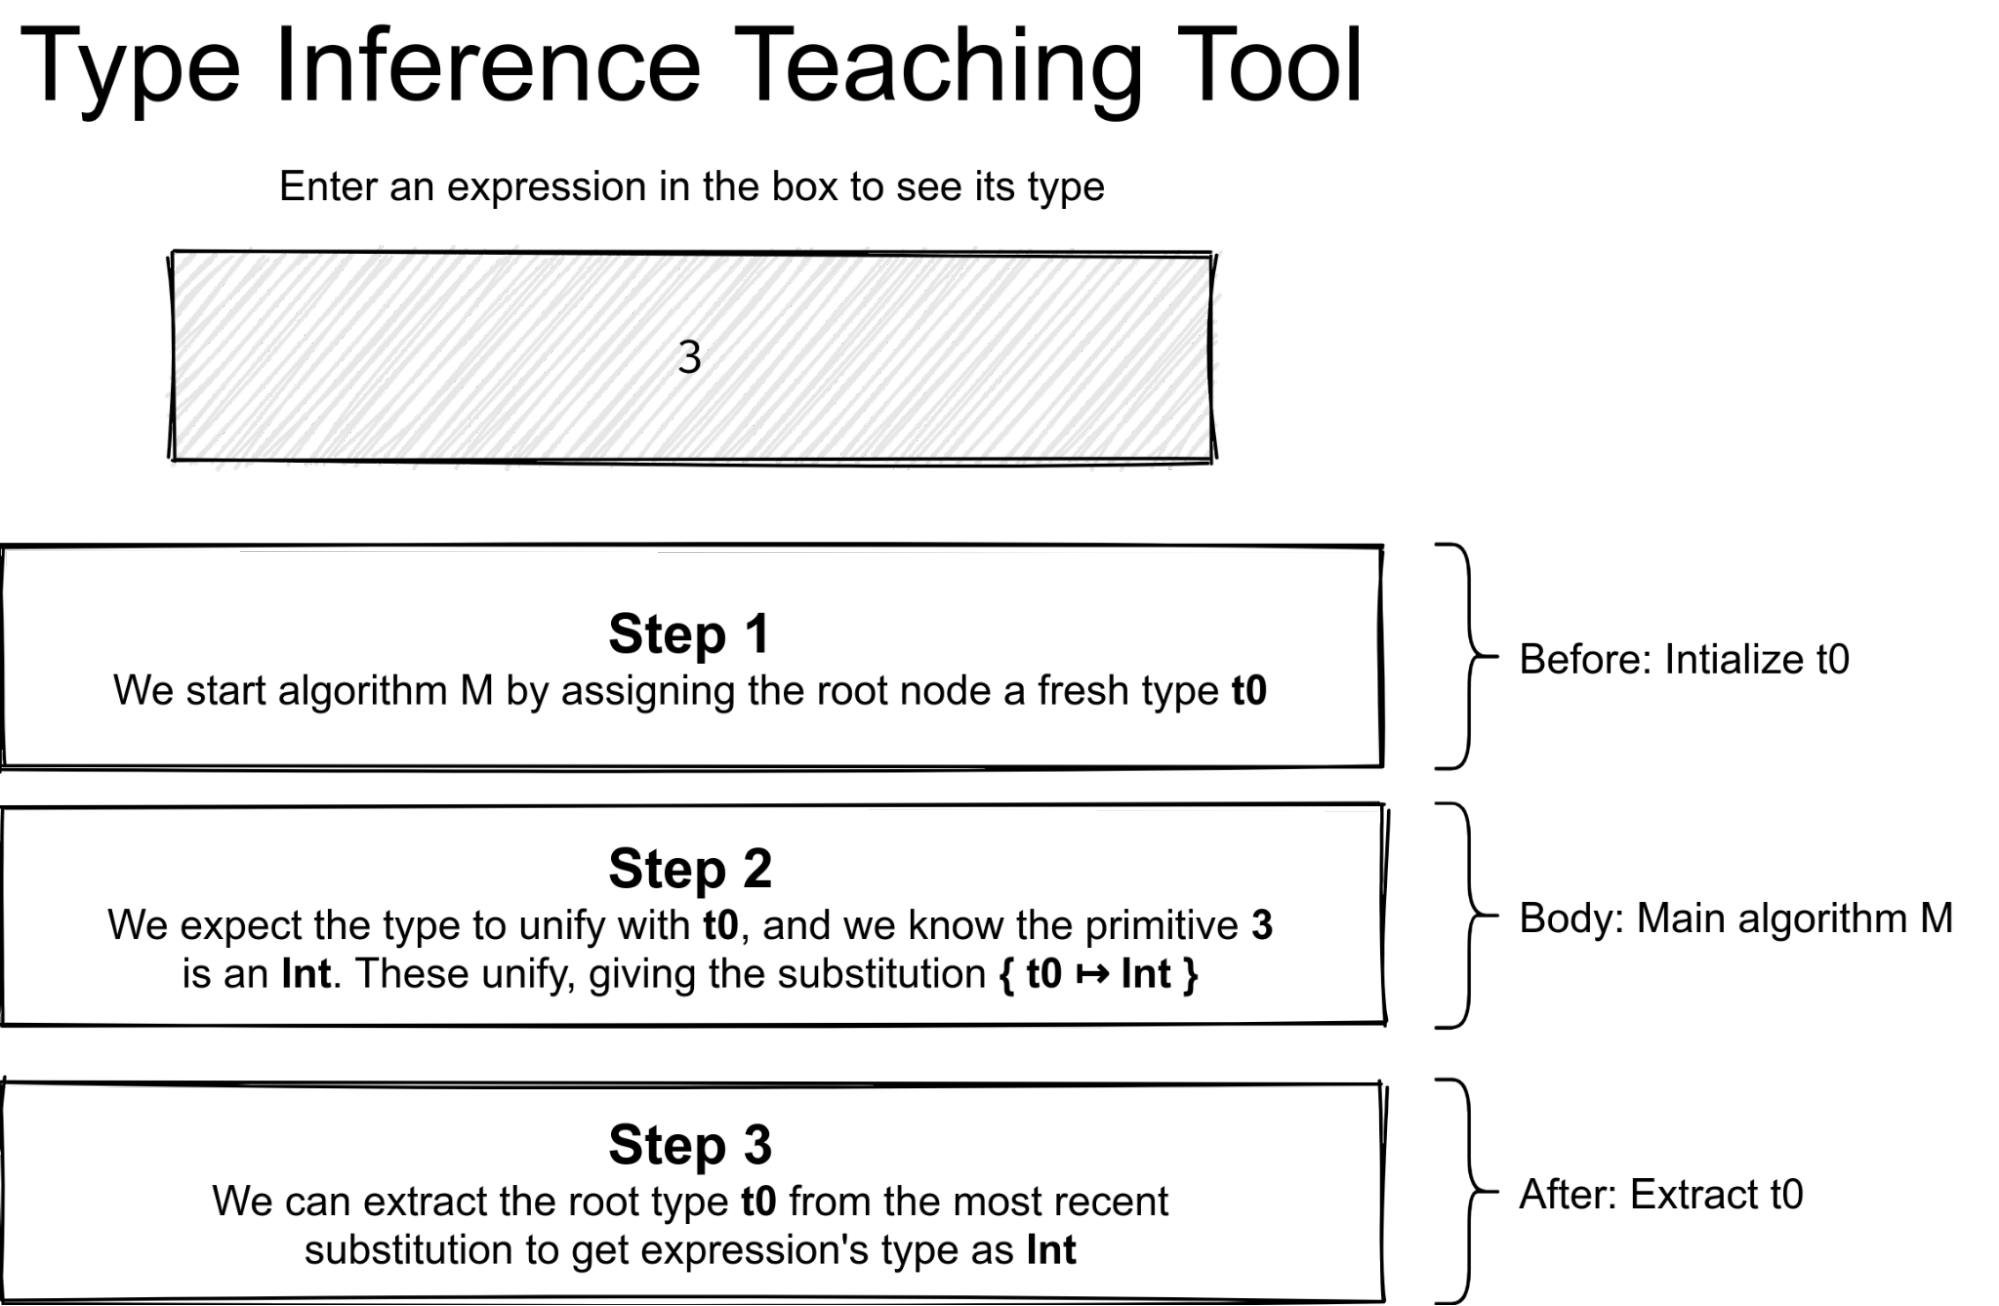
\includegraphics[width=0.960\linewidth]{images/image6.png}
  \caption{Algorithm M requires an initial and final step.}
\end{figure} \par}

To make it clear what part of the expression each step relates to, a representation of the expression as an AST with the relevant parts highlighted is shown at each step. The visualisation is computer generated and must fit in a fixed width space, and as such a vertical design was chosen to represent it. In this design, each box represents a tree node and the boxes are ordered in a vertical list. Nodes may have children, which they are attached to with edges to the left of the children.

{\centering \begin{figure}[h!]
  \centering
  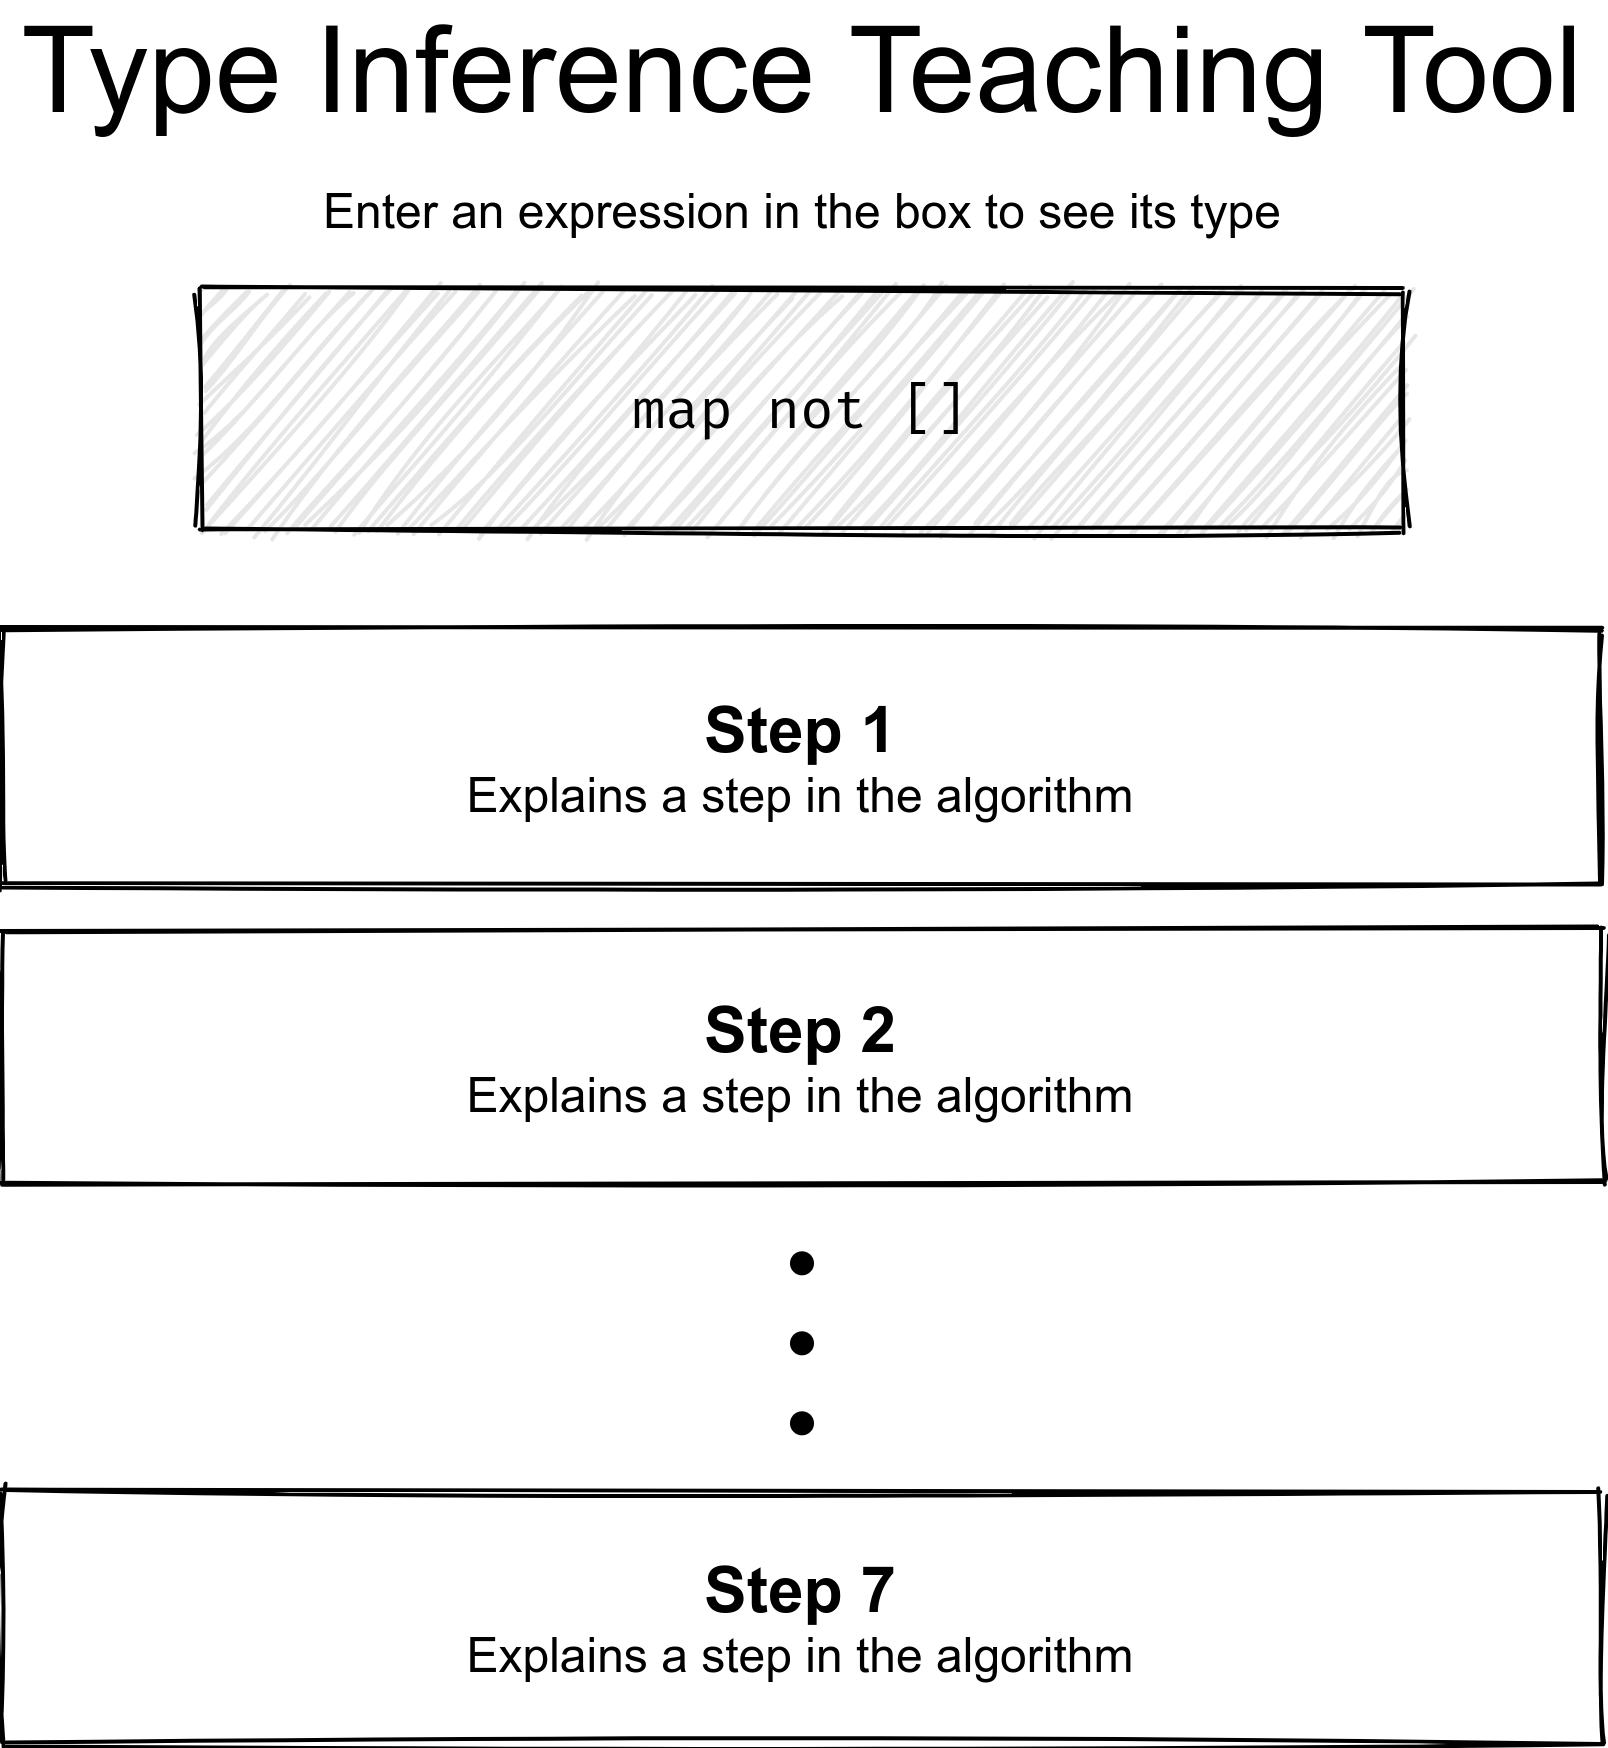
\includegraphics[width=0.357\linewidth]{images/image21.png}
  \caption{The expression \mintinline{text}{|let x = 3 in odd x|} may be represented by this vertical AST.}
\end{figure} \par}


This vertical design was chosen over a horizontal design due to the space constraints of the tool page, and the difficulty in implementing a consistent and well functioning horizontal tree visualisation algorithm.

{\centering \begin{figure}[h!]
  \centering
  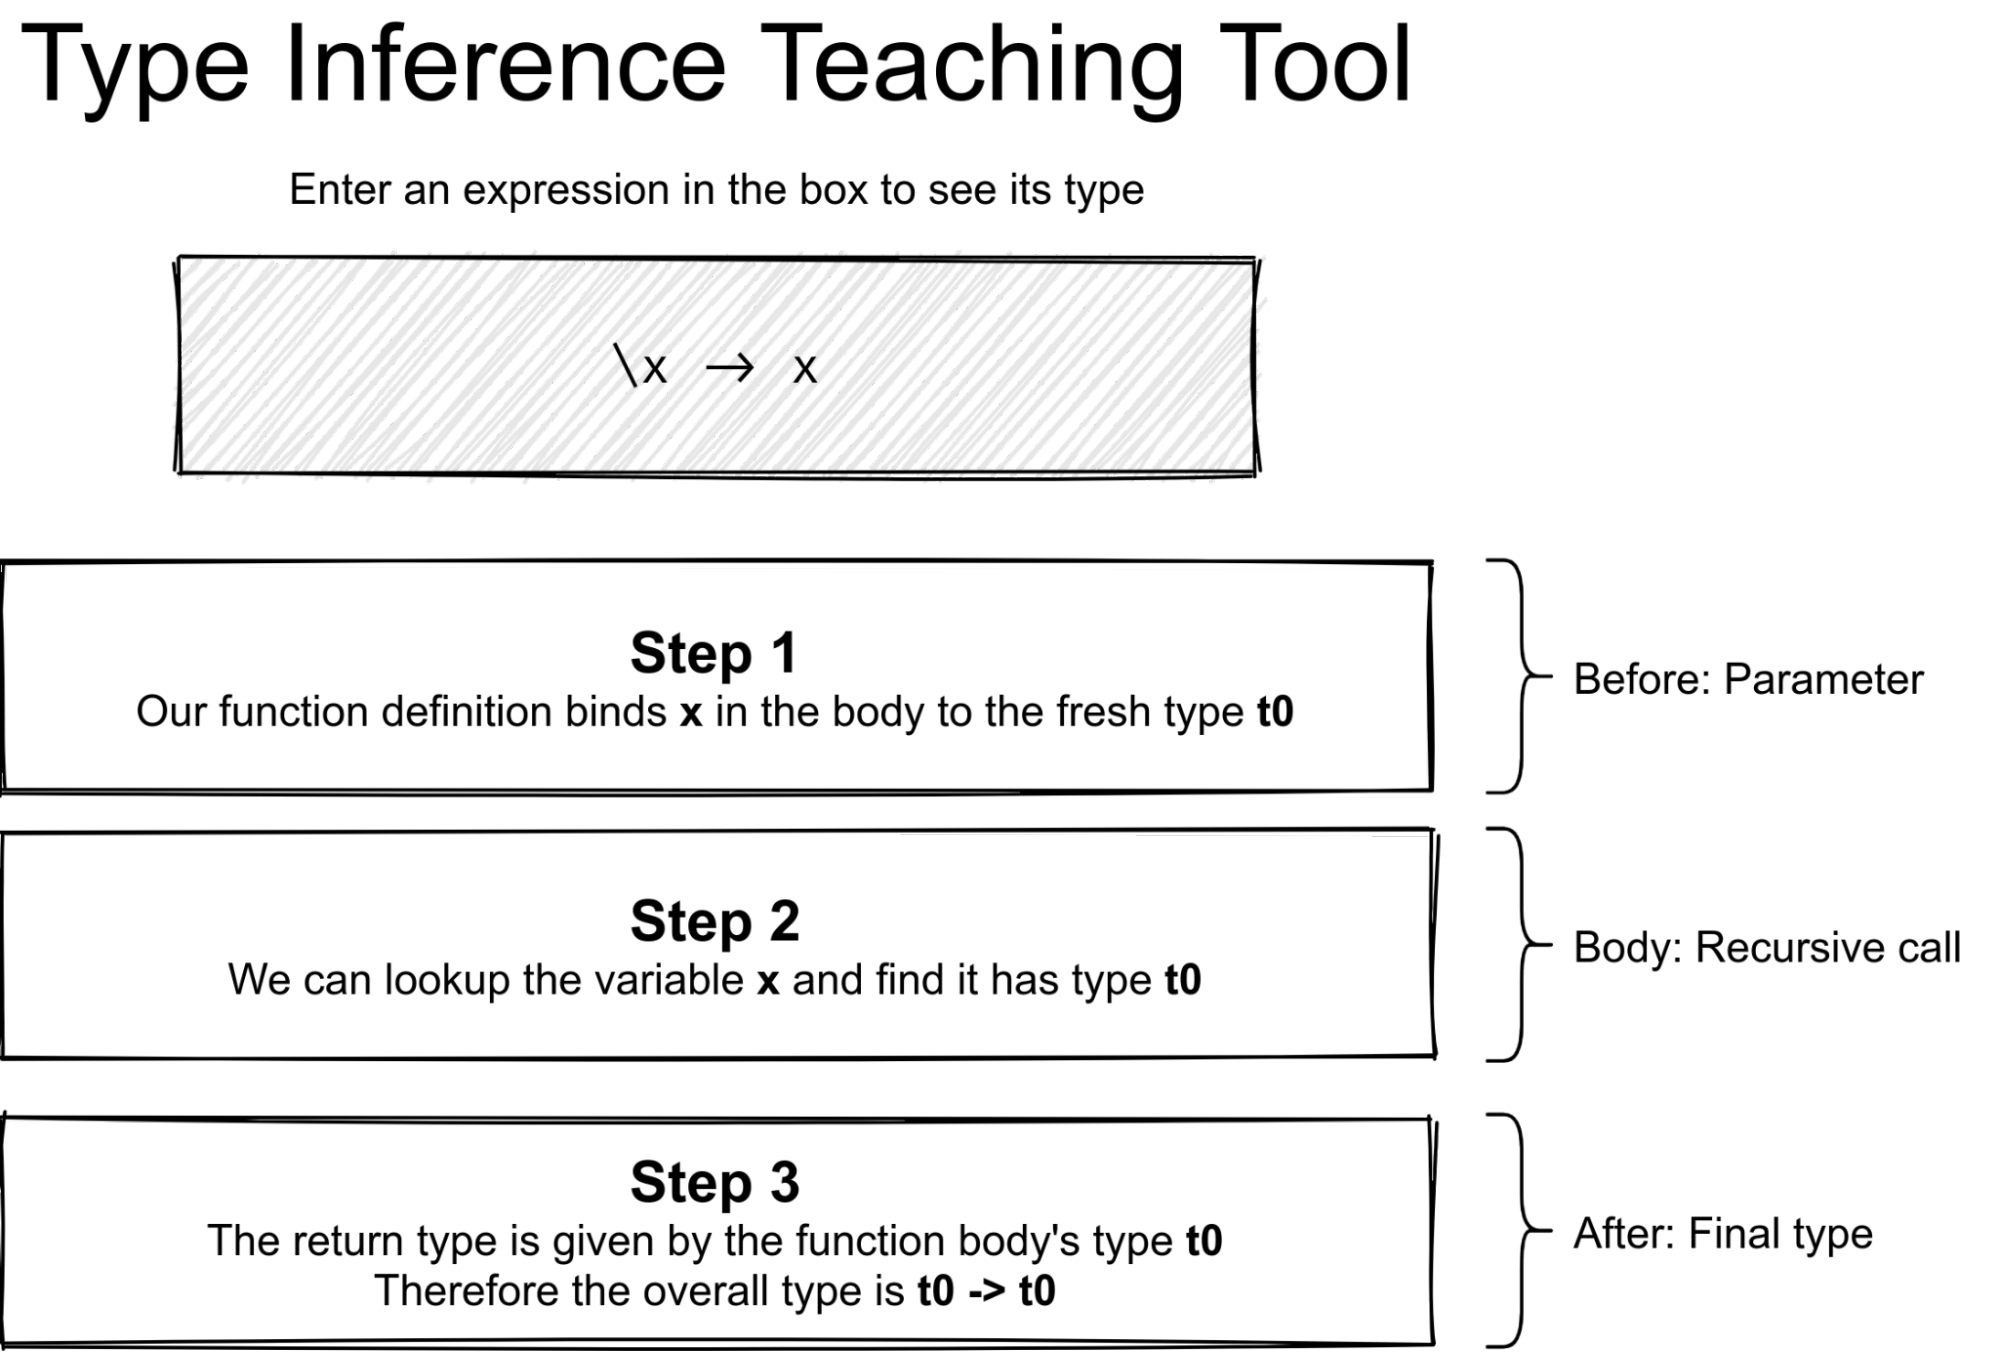
\includegraphics[width=0.813\linewidth]{images/image8.png}
  \caption{Example of what a more horizontal design of AST might look like.}
\end{figure} \par}

Showing ASTs is preferable to just showing the relevant subexpression as it makes it clearer what part of the whole tree is being analysed. Showing ASTs is also preferable to showing the full expression and highlighting only the relevant part as it better demonstrates how the program is broken into its constituent parts, is clearer for showing syntactically-sugared features such as lists, and relates it to the original type inference algorithms more closely as users can see how similar AST structures follow similar type inference rules.

To help relate the ASTs to the entered expression, when a user hovers over a part of the AST the matching part of the entered expression that corresponds to the hovered AST node is highlighted. For consistency and to help users understand larger subexpressions too this also works for non-leaf nodes of the tree.

{\centering \begin{figure}[h!]
  \centering
  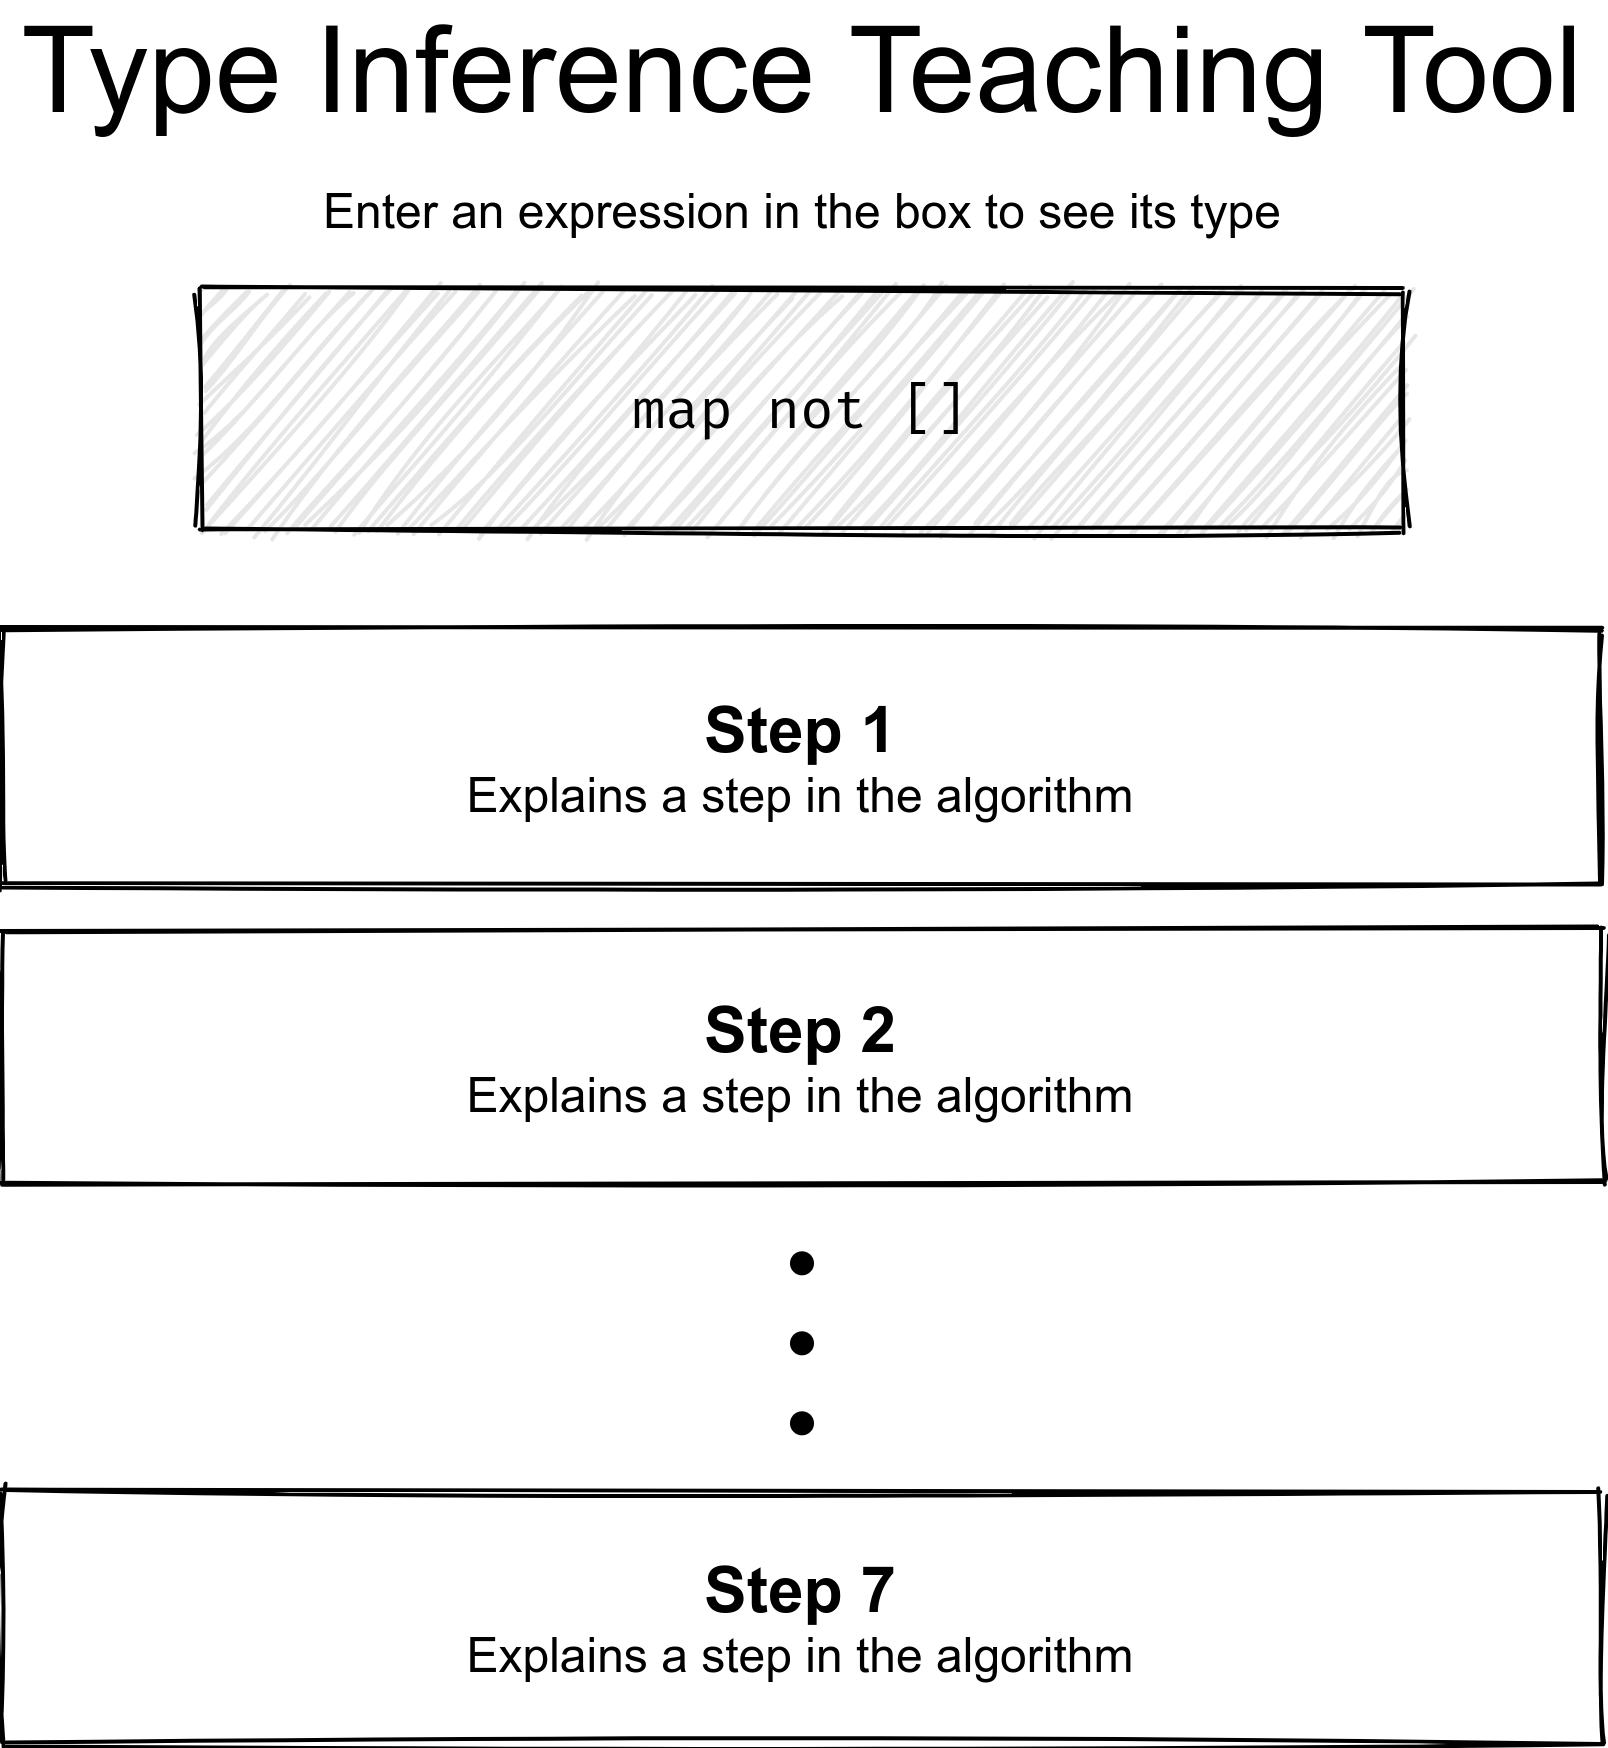
\includegraphics[width=0.884\linewidth]{images/image17.png}
  \caption{Hovering ove r the 'function application' node highlights the corresponding subexpression in the entered program.}
\end{figure} \par}

TODO: explain why web interface over desktop program
\subsection{Architecture}\label{id:h.l33hnjbawceh}
The design of the software aims to promote interchangeable, loosely-coupled modules to make it easy to adapt and extend. This also gives the project freedom to change over time in response to feedback, without having to redevelop common functionality.

TODO: insert module diagram

The alternative general module structure considered was to have the type inference modules standalone, to avoid depending on the language core. They would then be parameterized with methods to extract the necessary data from an arbitrary structured AST. This would allow the type inference algorithms to be used with any AST model. However, it would add significant complexity and performance overhead for not much gain as the language core is fairly lightweight. In addition, it would have meant utility functions, types and models could not be shared in the language core between type inference modules, meaning they would need to either have another separate module for shared utilities or have a large amount of code duplication.

TODO: insert alternate module diagrams

The main downside to splitting the project up into several modules is the tooling is a little more complex. Modules must be built separately and in the correct order which is slightly slower than compiling one larger app, and IDEs have to be set up to understand how to navigate between the modules. However, this is outweighed by the maintainability and extensibility benefits of keeping functionality in separate modules.

\subsubsection{Choice of programming language}\label{id:h.dj2rwwqr30vu}
All of the modules are written in the same language, so they are all compatible and easy to get working together. Additionally, using one typed language allows for type-checking to ensure module APIs are correctly called and their results are used sensibly. To write a modern web application, a JavaScript-compatible language is the obvious choice as it is supported and promoted by all major browsers. TypeScript was chosen for this for several reasons.

TypeScript is a statically-typed language similar to JavaScript which transcompiles to JavaScript that can be run in the browser. As a typed language, it provides the benefits of types listed earlier, which is especially important when dealing with a sizable codebase with several modules so was chosen over plain JavaScript.

Elm, CoffeeScript, PureScript and Dart are other languages that compile to JavaScript, however they lack rich package systems which can provide useful utilities and dependencies. Furthermore, Dart and Elm are largely focused on the presentation of data, so while it would be possible to write reusable independent libraries for type inference in them, it would not be easy.

Of the browser-compatible languages, TypeScript is the most used after JavaScript itself (according to the StackOverflow developers survey) and so developing and publishing packages in TypeScript may be useful for a wider audience.

Lastly, my own previous experiences with both TypeScript and the other languages informed the decision. Familiarity with TypeScript played a key role in choosing it over other languages targeting the browser.
\subsubsection{Language core}\label{id:h.hggmfighusoc}
The base module of the software, which all other parts depend on is the language core.

The language core contains key types and models, which are used throughout the rest of the software. These types and models are used in representing AST nodes, types, contexts, substitutions and other results from type inference algorithms. They also include function signatures which define the interfaces for modules containing type inference algorithms.

In addition to these types and models, it contains a default global context with types for many common functions. This context is based on Haskell’s Prelude, which makes it easy for learners familiar with Haskell or similar functional programming languages to use the tool.

The language core also contains key helper functions such as utilities to create types. For example, callers can construct and instance of a type as \mintinline{text}{|tuple(char, boolean)|} instead of \mintinline{text}{|new TypeFuncApp(‘,’, new TypeFuncApp(‘Char’), new TypeFuncApp(‘Bool’))|}. It also contains helpers to combine and apply substitutions, as well as to perform unification. These helper functions can be tested independently, verifying the correctness before using them in dependent modules. Testing is discussed in more detail in the implementation chapter.

Lastly, the language core contains a lexer and parser. Together, these take an input program as a string and return an AST, or report that the program is syntactically invalid. The lexer splits the input string into tokens, while the parser operates on this stream of tokens to recognise higher-level program constructs and construct the AST nodes.

A parser combinator library is used to perform the lexing and parsing. A parser combinator library was chosen over a recursive descent parser or an LL, LR or LALR parser generator as it was recommended by my project supervisor and several online sources discussing implementing functional language parsers. In addition the software needs to be compatible with running in the browser which most LL, LR and LALR generators do not support. In addition, none of these types of generators provides output that is easy to implement for the browser or debug manually, whereas parser combinators are relatively easier to implement by hand.

The library chosen for lexing and parsing is Masala, one of the few parser combinator libraries implemented in JavaScript. Masala is based on Haskell’s Parsec library, is tested for the browser and is well-maintained. In addition, it has strong TypeScript definitions which support its integration into the language module. Other libraries including Parjs, Parsimmon and Chevrotrain have weaker documentation, and Parsimmon lacks full TypeScript type definitions. Some other libraries like Jison and Nearley cannot easily and directly output the custom AST node classes, while Masala can. This helps extract the location of nodes in the source program to support being able to highlight where in the input expression an AST node has come from.
\subsubsection{Type inference algorithms}\label{id:h.75leuokwbltp}
On top of this language core are type inference algorithms W, W’ and M. Given an AST representing an expression, they return either a type or an error explaining why they were not able to infer the type. Along with these, they can also optionally return a sequence of steps taken as part of the algorithm. Each step includes a message and AST to be displayed, with appropriate parts of the AST highlighted.

Each type inference algorithm shares the same interface, allowing them to be used interchangeably. This means new algorithms conforming to this interface can be added to tools using the type inference algorithms, such as the web application, by simply changing the type inference library installed. Sharing the same interface also means that high-level module tests that call only the common function signature and assert on the final type can be shared across all the inference algorithms as they should all return the same type result, even if they take different steps to get there. This makes the development of tests easier so more can be written, and asserting the final types are the same across a number of varied cases improves confidence that the algorithms are implemented correctly.

Publishing the type inference algorithms separately helps keep the code clean and maintainable, and allows developers to only install the algorithms they need. While this does result in some code duplication, particularly between algorithm W and W’, the benefits from keeping the modules small and easier to maintain individually make this trade-off worthwhile. Most of the common helper functions are already in the language core, which means the code duplication in the type inference modules is not excessive.
\subsubsection{Web interface}\label{id:h.q67ivlz7h61r}
Finally, depending on both the language core and the type inference algorithms is the web interface itself. This is the end-product that users interact with, implementing the user interface. Here users can type in a program, and view the steps the type inference algorithm took to infer its type. To do this, the web application passes the program to the language core which lexes and parses it into an AST, then passes that AST to a type inference library. The results of this are then shown to the user.

TODO: diagram of pipeline: user enters program as string, lexer lexes as tokens, parser parses to AST, type inference algorithm returns steps, web application displays them

The web application uses the React framework. Using a framework improves the structure of the code, as the application can be broken down into separate, independent components. These components can be reused to minimise code duplication, and can be individually unit tested with many testing libraries developed specifically for frameworks. As well as this, using a framework in combination with a module bundler such as webpack makes importing and depending on other modules (such as the language core and type inference algorithms) simple. And in combination with a transcompiler that converts modern JavaScript to be backwards compatible, such as Babel, the application can be made to work for users with older browsers.

React was chosen over the alternative web frameworks Vue, Angular and Svelte. Vue and Angular are other popular frameworks, however for a one page application they are a little more complex than what is needed. In particular, Angular’s component and dependency injection system, while useful in very large projects, would add significant unnecessary overhead to developing the system. Svelte is different to React, Vue and Angular in that it avoids managing a model of the page through a framework library that is part of the application, but instead compiles directly to simple JavaScript. This gives it better performance, but makes it harder to integrate with existing libraries and tooling. In addition, while Svelte supports TypeScript this support was only added recently (July 2020) and is much weaker than React’s TypeScript support. Vue, Angular and Svelte are all significantly less popular than React (which is the most popular JavaScript framework). This means they have fewer available compatible packages and less community-developed documentation such as tutorials, guides or forums. In particular, Svelte is a new and much less widely-used framework, with less than 2,000 questions on StackOverflow compared to React’s nearly 300,000.

Create React App sets up the initial structure of the web application. It includes a starter template, which is set up with the required dependencies to build a basic React site. A variant of the starter template is available with TypeScript support. Using this starter template rather than starting from scratch allows the project to focus on developing the novel type inference teaching tool parts of the web application, rather than being too concerned with the setup of the tooling. However, using Create React App does somewhat limit how the build can be configured without choosing to “eject” (an irreversible process that makes the implicit build tooling explicit, but results in more maintenance). For example, while it installs Webpack and Babel to bundle resources and transcompile to more-compatible JavaScript, their corresponding configurations cannot be edited without an “eject”.

The web application directly imports the type inference algorithms and the language core, and bundles them as part of the client application to be run entirely inside the user’s web browser. Using a static site and doing the processing fully client-side was chosen over a client-server architecture to reduce latency, minimise running costs and maximise the resource’s longevity. It also helps to simplify communication between the modules, which otherwise would either need to be manually specified or use a complex networking layer, likely using the proxy pattern along with dependency injection. In addition, potentially complex data types representing the AST would otherwise need to be reliably serialized and deserialized which is non-trivial when as classes they have non-serializable member functions.

Performing calculations client side reduces latency as users do not need to wait on the network to transport data back and forth. Parsing and inferring the type of simple expressions in the browser takes tens of milliseconds, compared to the hundreds of milliseconds that might be expected from a RESTful API. However, for particularly complex expressions where users have particularly weak hardware (such as older smartphones) relative to the hosting server, doing calculations client-side may be slightly slower than a client-server architecture. These cases will be rare, but happen when the networking-related overheads are outweighed by the difference in processing speeds between the server and client devices.

TODO: insert bar graph comparing average laptop, average phone, average server-client, older smartphone, high latency server-client

Avoiding dynamic calculations on the server means free static hosting sites such as GitHub pages can be used to serve the website. This significantly reduces running costs when compared to running a custom server to respond to requests.

The teaching tool’s longevity is increased by serving a static artifact, as opposed to having dynamic server and client parts. A static website can easily be copied and archived, and as it can be run for free there is no incentive to shut the service down. TypeTool, a related work that also aimed to explain type inference, was client-server based. However, the server has since been taken down and so is no longer accessible. As the lexing, parsing and type inference process was done server-side, archive websites like the Internet Archive’s Wayback Machine are unable to keep a copy of it, as they only store the static website content.
\subsection{Analytics}\label{id:h.60njhv340fb0}
To help evaluate the main teaching tool and understand user behaviour, a system to collect and store behavioural analytics data is required. This tool should respect user privacy settings, minimize personal data collected (ideally data collected should be anonymous) and be able to view a single event stream to understand how a user is using the application.

Several of the most popular existing analytics solutions were explored, including Google Analytics, Matomo, W3Counter, Simple Analytics, Angelfish, Open Web Analytics and AWStats.

The “Do not track” (DNT) browser setting is the simplest and most widely-supported way to indicate a user does not want to be tracked. However, Google Analytics, Angelfish, W3Counter, Open Web Analytics and AWStats do not respect “do not track” browser settings by default, and while possible are difficult to set up so that they do.

IP addresses are classified as personal data under the General Data Protection Regulations (GDPR). Some analytics tools such as Angelfish, AWStats, Open Web Analytics and W3Counter collect and analyse IP addresses and other personal data. This presents a problem for using these analytics tools within the EU, as users must be informed as to how their personal data is collected and processed, and users have several rights relating to personal data such as the right to be forgotten, the right to object or the right to access. In addition, many of these tools use cookies and similar on-device storage technologies to track users, which require consent under the UK’s Privacy and Electronic Communications Regulations (PECR). This would add significant unwanted overhead to the website for what is actually necessary.

To understand user behaviour, a single event stream that shows the different steps they took would be most useful. For example, seeing in what order they try out type inference examples and whether they view the more in depth documentation is much more useful data for evaluating and improving the tool than aggregate data about user demographics. Many platforms such as AWStats focus on the latter, and do not offer event stream (also known as ‘clickstream’ or ‘clickpath’) analytics. Some platforms meet in the middle, offering event tracking but cannot present these in individual user streams such as Google Analytics. Angelfish offers event stream analytics, but does not support custom events, such as choosing a type inference example.

Finally the most practical concern is their running cost. Google Analytics and W3Counter are the options with free plans, while other managed services such as Matomo Cloud and Simple Analytics are generally fairly expensive (both more than £275 per year for their cheapest plan). The cheapest available Angelfish license costs over £1,000 a year, and along with “free” options AWStats and Open Web Analytics needs to be hosted on a server which would incur server running and maintenance costs.

These factors can be summarised in a comparison table:



\begin{adjustbox}{center}\begin{tabular}{ |l|l|l|l|l| }
  \hline
  \textbf{Service} & \textbf{Obeys DNT} & \textbf{Anonymous} & \textbf{Event streams} & \textbf{Cost} \\
  \hline
  Google Analytics & ✗ & ✗ & ✗ & Free \\
  \hline
  Matomo Cloud & ✓ & ✓ & ✓ & £348/year \\
  \hline
  Matomo (self-hosted) & ✓ & ✓ & ✓ & Server hosting \\
  \hline
  W3Counter & ✗ & ✗ & ✓ & Free \\
  \hline
  Simple Analytics & ✓ & ✓ & ✓ & £276/year \\
  \hline
  Angelfish & ✗ & ✗ & ✓ & £1123/year + server hosting \\
  \hline
  Open Web Analytics & ✗ & ✗ & ✓ & Server hosting \\
  \hline
  AWStats & ✗ & ✗ & ✗ & Server hosting \\
  \hline
\end{tabular}\end{adjustbox}\\

From this, we see that self-hosted Matomo is the only somewhat affordable option considering the budget for a 3rd year project. However, Matomo’s set up is complicated and managing and maintaining a server is time-consuming. In particular, ensuring data is held securely would require running or renting a potentially-expensive private server indefinitely for hosting, as the available free departmental machines such as Joshua do not guarantee confidentiality, integrity or availability. The departmental machines also limit the installation of certain software which require root permissions, and many applications are not supported as Joshua libraries are outdated. In addition frequent restarts combined with limited powers to automatically run applications (through systemd units or similar) on Joshua means Matomo would have to be frequently restarted manually and may miss some user events.

As such, we design a custom analytics platform to meet the three main criteria while having a very low running and maintenance cost.

This platform offers an API to record custom events. The web application is then augmented to call the API to log certain user behaviours such as opening the help section or viewing a type inference example. An anonymised identifier is created for each new visit, which allows events to be collected and later viewed in anonymised custom event streams.

The data collected is the anonymised identifier, a timestamp, and any payload specified by the web application. For example to represent a user choosing to show the more detailed helper a JSON payload may be sent, such as:

\begin{minted}[breaklines]{json}
\{ "name": "help", "value": "show" \}
\end{minted}

Or, in the case where an button to set up the code example \mintinline{text}{|map not []|} the web application may send the payload: 

\begin{minted}[breaklines]{json}
\{ "name": "codeButtonSet", "value": "map not []" \}
\end{minted}

The analytics API records this data, associating it with the anonymised identifier and timestamp. This is held securely for a configurable retention period, which is by default set to 90 days. While there are no legal requirements or responsibilities under PECR or GDPR to hold this data securely and minimize data retention as it is not personal data, doing so follows best ethical practices and reducing the volume of data held reduces running costs.

Running costs generally are kept low (<£1 per year) by using serverless cloud products. These are cloud products which offer compute and storage in individual on-demand units, rather than requiring renting of a permanent server. Serverless products also allow the analytics platform to easily scale to handle spikes in traffic, while being free when the site is not in use.

The custom event streams are then viewed in an analytics viewer. To keep the implementation consistent between the main project and the analytics sub-project, this too is written as a TypeScript application initialized with Create React App. Using a different framework would have resulted in less knowledge sharing between the two, and introduced additional unwanted complexity. Also, for similar reasons to the main project React was a well-suited framework for the viewer.

\begin{figure}[h!]
  \centering
  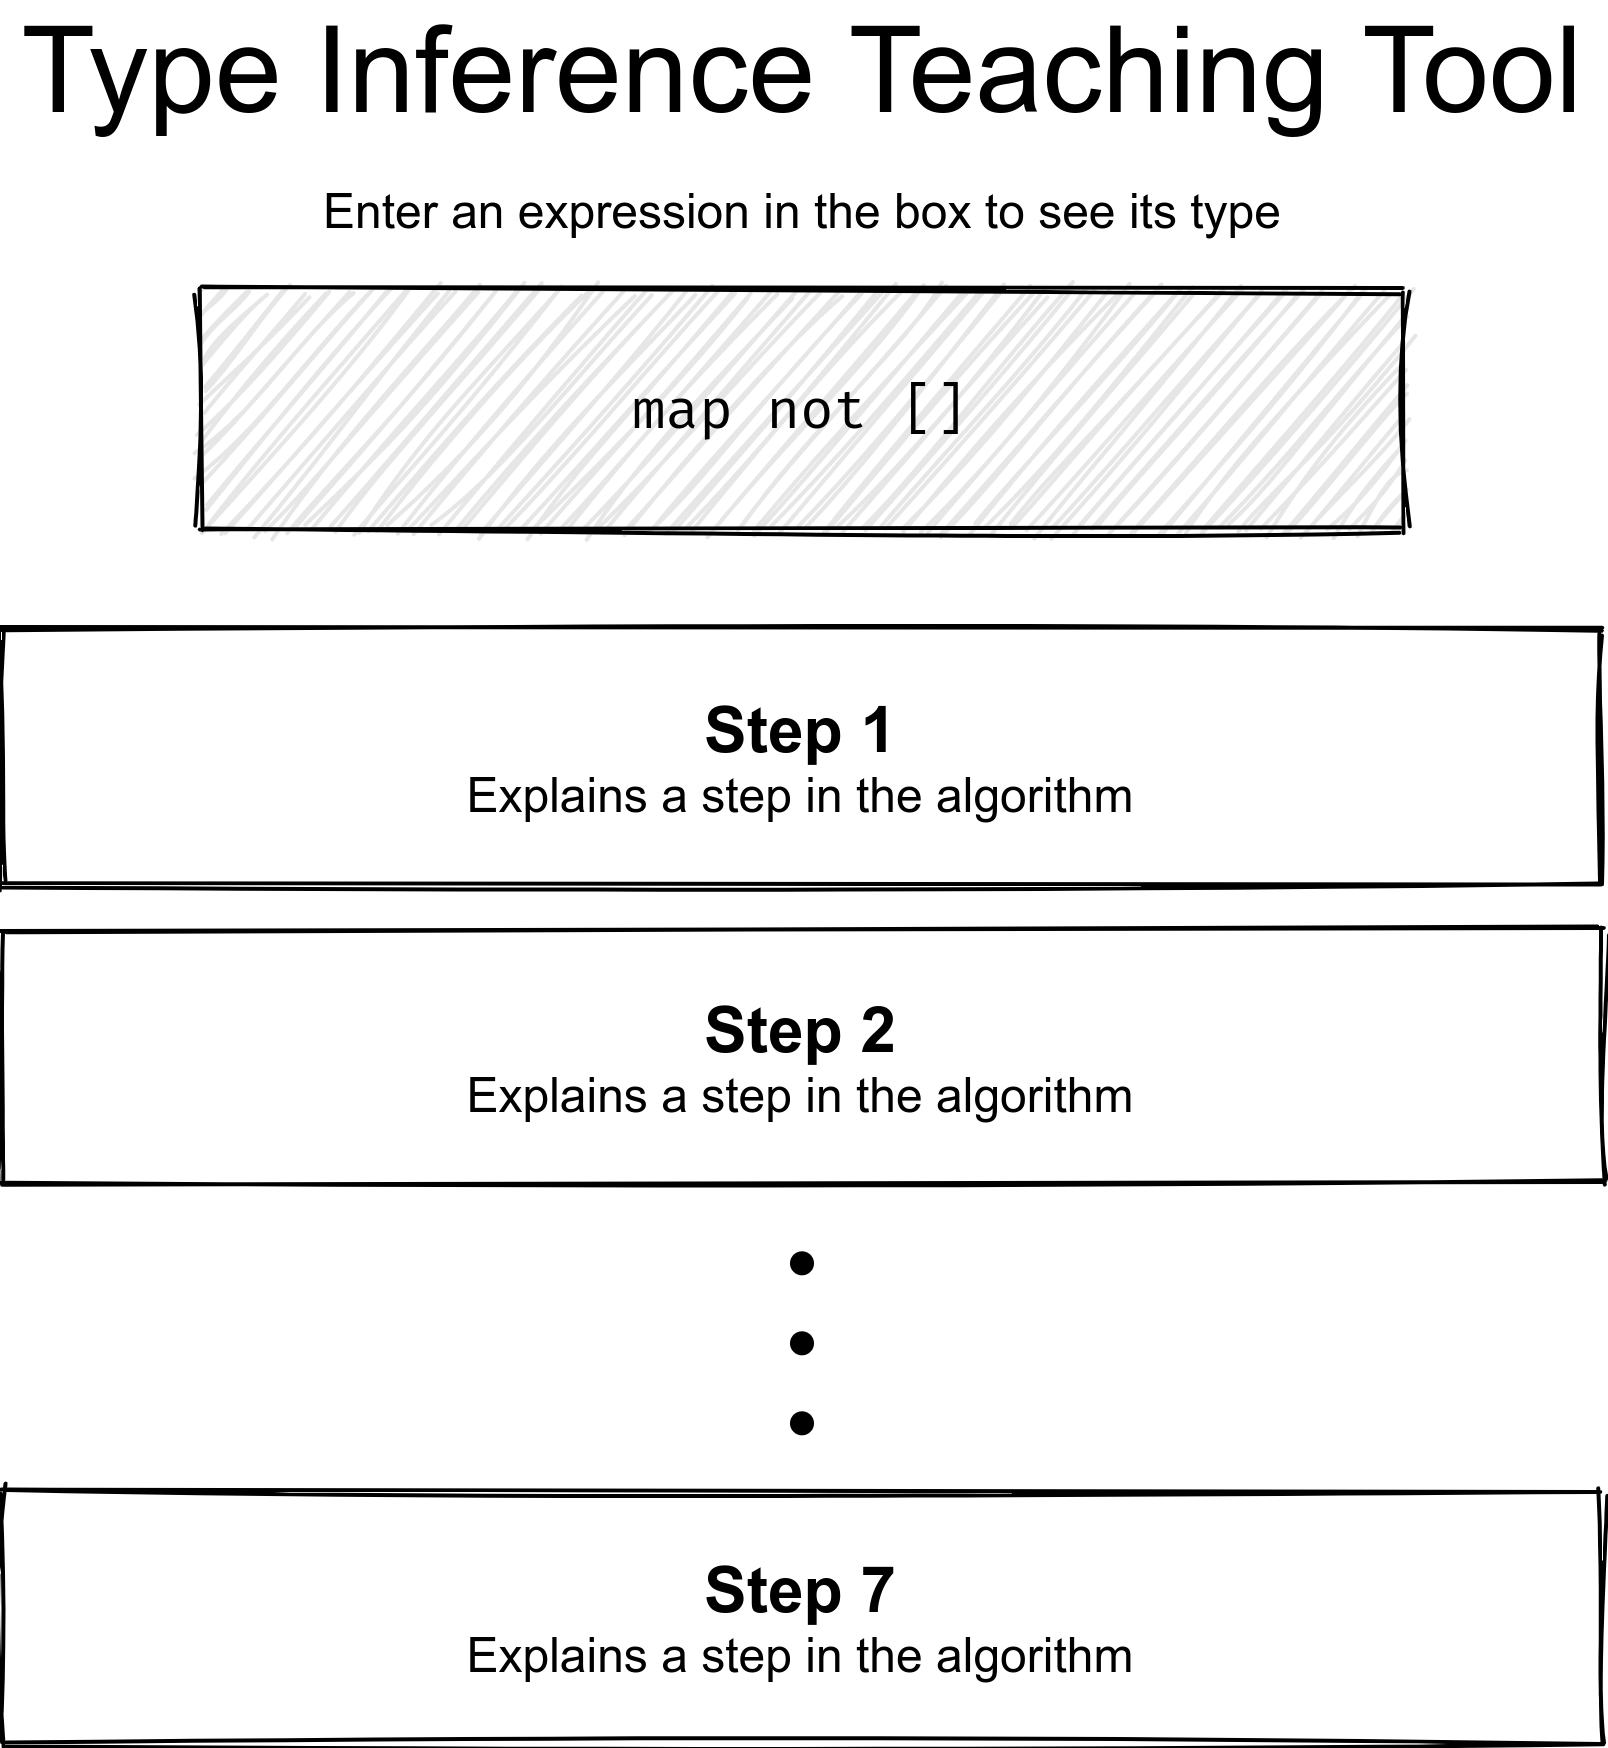
\includegraphics[width=1.000\linewidth]{images/image10.png}
  \caption{The analytics viewer, showing an example stream from the web application.}
\end{figure}

The viewer shows analytics events by stream, which can be navigated simply using the left sidebar which represents a list of streams. The main view shows a list of events within that stream, ordered by timestamp.
\section{Implementation}\label{id:h.igepudpadp49}
As detailed in the design section, the application is broken into several loosely-coupled modules, written in TypeScript. This chapter details their implementation, examining specific features of the code at a lower level.

\subsection{Language core}\label{id:h.o3ngfa303saw}
The language core contains models, utility and helper functions, and a lexer and parser. Together these comprise all the basics for interpreting and representing the expression language, and support implementing the type inference algorithm upon it.

For clarity, in this section the term ‘models’ will be used to mean TypeScript types, function signatures, interfaces and classes. The term ‘types’ will be used exclusively to refer to the type objects, used for example as the result of type inference algorithms. For example the TypeScript expression in the implementation:

\begin{minted}[breaklines]{typescript}
new TypeVar(‘t0’)
\end{minted}

instantiates a TypeVar \textit{model} that represents the \textit{type} $t0$.
\subsubsection{Models}\label{id:h.f0aymht9bwx3}
TypeScript models are used to represent abstract syntax trees, types, contexts, substitutions, results and errors.
\subsubsubsection{Abstract syntax trees}\label{id:h.26q0jf334v10}
Abstract syntax trees are represented by their nodes alone. Each node corresponds to a subexpression, and contains the relevant information about itself and has references to its direct children. For example, the AST for the expression \mintinline{text}{|\x -> not x|} may be represented by the node:

{\centering \begin{figure}[h!]
  \centering
  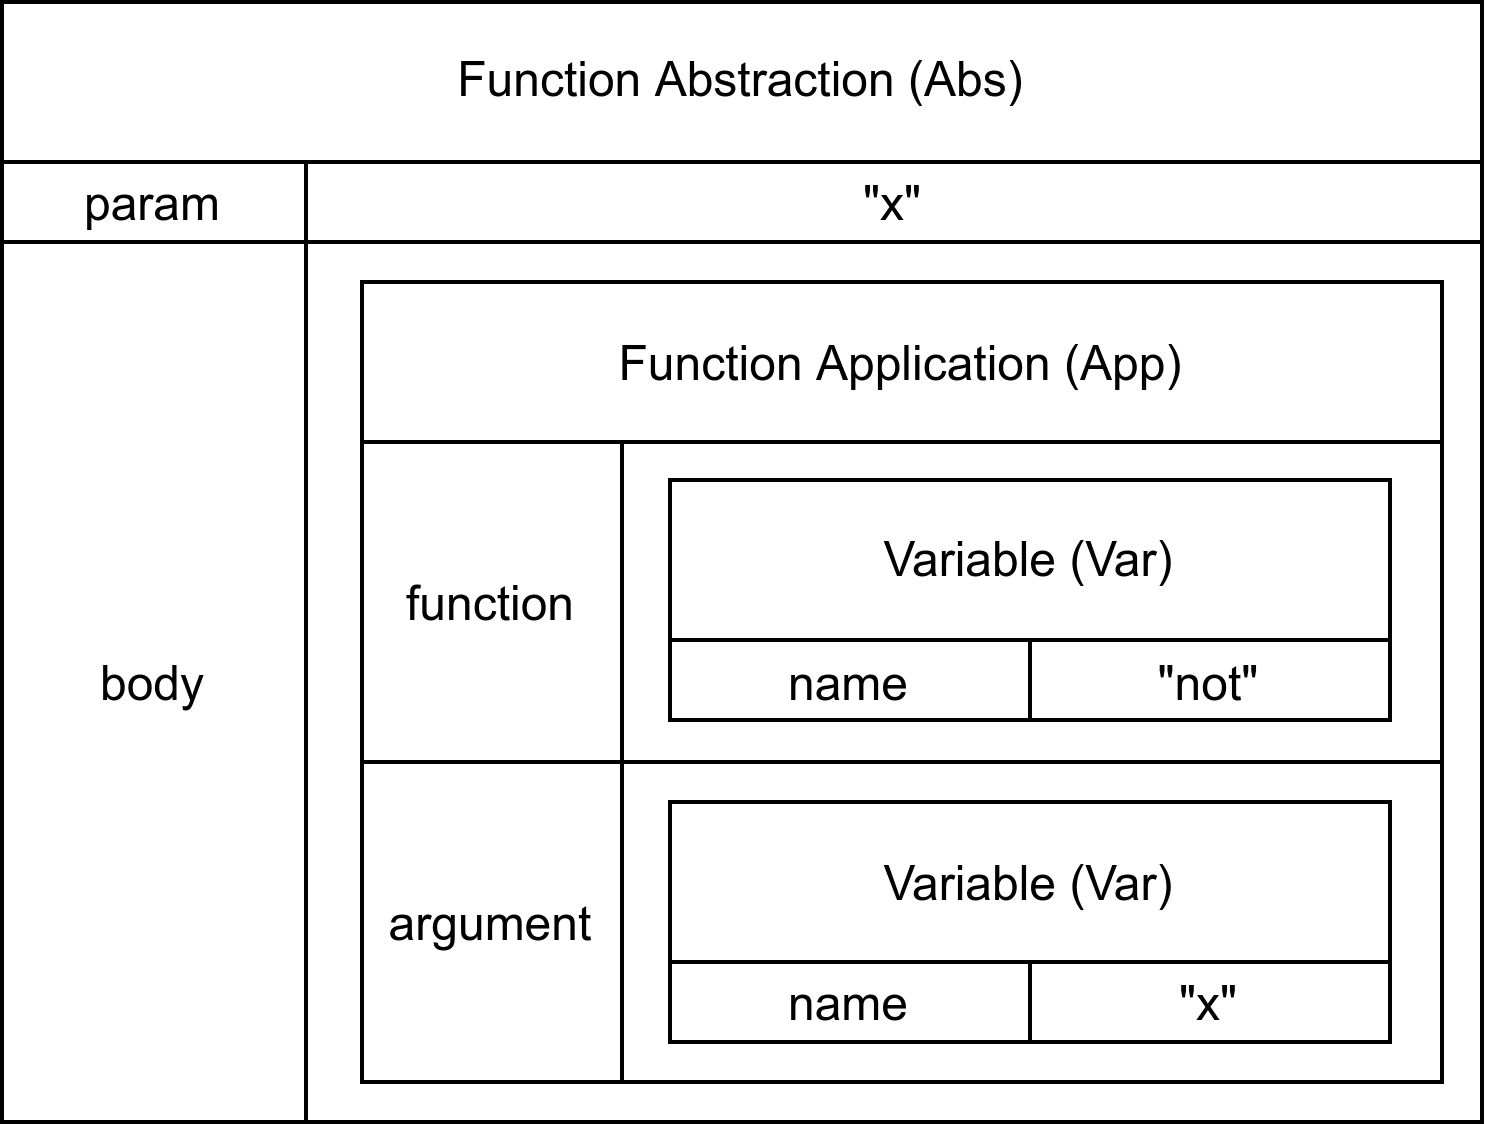
\includegraphics[width=0.863\linewidth]{images/image12.png}
\end{figure} \par}

Here we see the tree is effectively just an \mintinline{text}{|Abs|} node, with a \textit{parameter} by the name of “x” and \textit{body} with a reference to another AST node. This body node is an \mintinline{text}{|App|} node, which has two properties: a \textit{function} and \textit{argument}, each being AST nodes of type \mintinline{text}{|Var|}. These \mintinline{text}{|Var|} nodes have a single property \textit{name}, the name of the variable referenced.

All nodes represent some expression in the original program. We declare a model \mintinline{text}{|Expr|} as the union of all the different node models, which we can use to represent a general subtree. This is used in defining the node models, for example in its simplest form the \mintinline{text}{|Abs|} node in TypeScript can be represented:

\begin{minted}[breaklines]{typescript}
interface Abs \{
  param: string;
  body: Expr;
\}
\end{minted}

To expand upon this model, we add the position in the original source program it was found at. This can be represented by a simple start and end index into the string of the source program, where the start is the index of the first character (0-indexed) and the end is the index of the last character plus one. For example, the \mintinline{text}{|Var|} node representing \mintinline{text}{|not|} in \mintinline{text}{|\x -> not x|} starts at index 6 and ends at index 9. This indexing scheme is convenient as the length of the expression in the original source code can be calculated by simple subtraction, and the standard TypeScript string methods \mintinline{text}{|slice|} uses this convention. Therefore \mintinline{text}{|code.slice(p.start, p.end)|} will result in the source code specified by a position \mintinline{text}{|p|}. Positions are represented by the simple model:

\begin{minted}[breaklines]{typescript}
interface Position \{
  start: number;
  end: number;
\}
\end{minted}

In addition to positions, AST nodes have a notes property. This is represented as an optional string, and is used to record additional arbitrary information about certain nodes, for example that they should be highlighted in the UI or that they are from certain syntactically sugared expressions. For \mintinline{text}{|Abs|}, we now have:

\begin{minted}[breaklines]{typescript}
interface Abs \{
  param: string;
  body: Expr;
  pos: Position;
  notes?: string;
\}
\end{minted}

Once constructed, properties should be immutable. Immutability prevents properties from being changed, which prevents certain hard-to-detect bugs as all object transformations must be explicit. For example, a method call to an object may not unexpectedly change that object. In addition, immutability helps . While immutability may have a small performance and memory usage overhead in some implementations, this may be offset (and in some cases, performance may be improved) by structural sharing. Structural sharing uses existing references to parts of an object when making a slightly changed copy of it. This reduces memory usage and reduces the overhead of creating new objects. This can be done safely given the knowledge objects are immutable as neither reference will attempt to update the child. For example:

TODO: diagram

Finally, immutability can improve performance when using front-end frameworks like React, which is used to implement the web application. With immutability, front-end frameworks can be sure objects have not changed on subsequent renders if they have referential equality (they point to the same object). Without immutability, objects may have changed between render calls so the front-end framework must re-render the page or perform deep value equality comparisons which require traversing the entire object. These are both potentially costly operations, so avoiding them through immutability brings performance benefits.

TODO: discuss use of const and let

Given the benefits of immutability, models are updated to generally be immutable, marked with the \mintinline{text}{|readonly|} modifier in TypeScript:

\begin{minted}[breaklines]{typescript}
interface Abs \{
  readonly param: string;
  readonly body: Expr;
  readonly pos: Position;
  readonly notes?: string;
\}
\end{minted}

To make constructing these models easier, we convert these TypeScript interfaces into classes. This allows us to use the \textit{new} keyword to construct instances of these models, and we can use the \textit{instanceof} operator to verify an AST node is of a specific type more easily. These are not possible with TypeScript interfaces alone.

In addition, classes allow us to easily add default methods to objects. We add a \mintinline{text}{|toString|} method to all AST node classes which returns a string containing a program representing the node. This then gives us the final implementation for our \mintinline{text}{|Abs|} node:

\begin{minted}[breaklines]{typescript}
class Abs \{
  readonly param: string;
  readonly body: Expr;
  readonly pos: Position;
  readonly notes?: string;

  constructor(param: string, body: Expr, pos: Position, notes?: string) \{
    this.param = param;
    this.body = body;
    this.pos = pos;
    this.notes = notes;
  \}

  toString(): string \{
      return '(\textbackslash ' + this.param + ' -> ' + this.body.toString() + ')'
  \}
\}
\end{minted}

This structure is used for all the AST node models, including:
\begin{itemize}
  \item \mintinline{text}{|Var|} for variables
  \item \mintinline{text}{|App|} for function application
  \item \mintinline{text}{|Abs|}, for function abstraction, as shown above
  \item \mintinline{text}{|Let|} for let statements
  \item \mintinline{text}{|CharLiteral|} and \mintinline{text}{|NumberLiteral|} for literal constants
\end{itemize}

\subsubsubsection{Types}\label{id:h.bzdo56ibho4h}
As discussed in the background chapter, monotypes are constructed from type variables and type function applications. We consider basic types (such as $Bool$ or $Int$) to be type function applications on zero arguments. Polytypes are monotypes with zero or more for-all quantifier variables.

For simplicity when modelling polytypes, we consider type variables bound at the highest level. Any type that can be expressed with for-all quantifiers at lower levels, is equivalent to moving those bindings to the top level. For example, $\forall a. (a \rightarrow (\forall b. (b \rightarrow (a, b)))$ is equivalent to $\forall a \forall b. (a \rightarrow b \rightarrow (a, b))$.

From this, and following the same reasoning about using classes with readonly properties we can develop simple models for types. Here we remove constructors and toString methods for simplicity.

\begin{minted}[breaklines]{typescript}
type MonoType = TypeVar | TypeFuncApp;

class TypeVar \{
  readonly name: string;

  /* constructor and toString methods */
\}

type TypeFunc = "->" | "[]" | "Maybe" | "Either" | "Int" | "Char" | "Bool" | "," | ",," | /* ... */;

class TypeFuncApp \{
  readonly constructorName: TypeFunc;
  readonly args: MonoType[];

  /* constructor and toString methods */
\}

class PolyType \{
  readonly quantifiedVars: string[];
  readonly monoType: MonoType;

  /* constructor and toString methods */
\}
\end{minted}

While PolyType’s \mintinline{text}{|quantifiedVars|} property could be modelled with \mintinline{text}{|TypeVar[]|}, for simplicity \mintinline{text}{|string[]|} was chosen as the methods on these type variables are never called.

The constructors are all trivial, and simply set the corresponding properties in the object. The \mintinline{text}{|toString|} methods are fairly simple for \mintinline{text}{|TypeVar|} and \mintinline{text}{|PolyType|}, however \mintinline{text}{|TypeFuncApp|} has additional logic to pretty-format some types. For example, it formats types like $[(Bool, Int)] \rightarrow Int$ rather than $\rightarrow ([] (, (Bool) (Int))) (Int)$ which would be the result if it treated all type functions equivalently in prefix notation with explicit bracketing. To do this it uses case matching, with different rules depending on the type function used.
\subsubsubsection{Contexts and substitutions}\label{id:h.ux3btyb2wvh8}
A context, as defined in the background chapter, is a mapping from variable names to their corresponding types. This informs the type inference algorithm what variables are in scope, and what their types are.

This is modelled in TypeScript as a simple object which has string keys (variable names) and type values. Specifically these type values are polytypes, because as stated before monotypes can be considered polytypes with zero for-all quantified variables. This is written:

\begin{minted}[breaklines]{typescript}
interface Context \{ [name: string]: PolyType | undefined \}
\end{minted}

Substitutions can be seen as mappings from type variable names to corresponding types they should be substituted with. In Hindley-Milner there is no need to ever substitute type variables with polytypes, so we can assume these are only monotypes. This therefore can be represented with a model similar to contexts:

\begin{minted}[breaklines]{typescript}
interface Substitution \{ [name: string]: MonoType | undefined \}
\end{minted}
\subsubsubsection{Results and errors}\label{id:h.5yk2zijb0axq}
The parser and type inference algorithms use response models to return their results. A \mintinline{text}{|Response|} from one of these methods may either be a \mintinline{text}{|Rejected|} or \mintinline{text}{|Accepted|}, indicating the input was invalid or valid respectively.

For example, if a syntax error is present in the program passed to the parser, it may return a \mintinline{text}{|Rejected|} model with the location of the error and a message explaining the issue. Alternatively if a valid program is passed to the parser, it returns an \mintinline{text}{|Accepted|} model with the AST representation as its value. Similarly, the type inference algorithms return \mintinline{text}{|Rejected|} if type inference fails, and \mintinline{text}{|Accepted|} if it succeeds.

These models are defined:

\begin{minted}[breaklines]{typescript}
type Response<A, R = undefined> = Accepted<A> | Rejected<R>;

interface Rejected<T> \{
  value?: T;
  accepted: false;
  issuePosition: Position;
  message: string;
\}

interface Accepted<T> \{
  value: T;
  accepted: true;
\}
\end{minted}

These models have generic parameters which can be used to specify the type of value expected to be returned. For example, an \mintinline{text}{|Response<Expr, ParseError>|} represents a model which may either be an \mintinline{text}{|Accepted<Expr>|}, containing an \mintinline{text}{|Expr|} as a value, or a \mintinline{text}{|Rejected<ParseError>|}, containing an optional \mintinline{text}{|ParseError|} as a value.

In addition to this, a \mintinline{text}{|TypeResult|} container is defined which is used as part of the function signature for type inference algorithms. This contains a type, representing the overall type of the expression, and the steps the type inference algorithm took to derive that type. Each step has a message and AST to go with it, to match the designed user interface steps.

\begin{minted}[breaklines]{typescript}
interface TypeResult \{
  type: MonoType;
  steps: \{ message: string, ast: Expr \}[];
\}
\end{minted}

Type inference algorithms return a \mintinline{text}{|Response|} where if \mintinline{text}{|Accepted|}, the value should be a \mintinline{text}{|TypeResult|} object. If \mintinline{text}{|Rejected|}, the value should be the steps only in the \mintinline{text}{|TypeResult|}. A TypeScript utility, \mintinline{text}{|Omit|} is used to remove the \mintinline{text}{|’type’|} property from the TypeResult in the rejection case. This gives the overall return type for type inference algorithms:

\begin{minted}[breaklines]{typescript}
Response<TypeResult, Omit<TypeResult, 'type'>>
\end{minted}

TODO: consider cutting/moving the following paragraph

In addition to these result wrappers, the parser and type inference algorithms also offer an alternative simple interface where just the AST or type is returned without any wrappers. In this case, if an error is found with the input a \mintinline{text}{|ParseError|} or \mintinline{text}{|TypeInferenceError|} is raised, which should be caught by the caller. These errors are also used internally by the methods returning result wrappers.
\subsubsection{Helper functions}\label{id:h.sw77qek8b49p}
Several helper functions are implemented in the language core that are relevant to the parser and type inference algorithms. Generally these perform the functions by the same name defined in the background chapter:
\begin{itemize}
  \item \mintinline{text}{|apply|} applies a substitution to a type or context
  \item \mintinline{text}{|combine|} combines substitutions
  \item \mintinline{text}{|unify|} attempts to find a unifying substitution given two monotypes
  \item \mintinline{text}{|contains|} returns whether a type contains a certain type variable
  \item \mintinline{text}{|freeVars|} returns an array of free variables names in a given type or context
  \item \mintinline{text}{|inst|} instantiates a type, replacing all for-all quantified type variables with new type variables
  \item \mintinline{text}{|generalise|} fully generalises a type, for-all quantifying any free type variables in the type that are not free in the given context
  \item \mintinline{text}{|unique|} removes duplicate elements from an array
  \item \mintinline{text}{|diff|} performs the list difference operation
\end{itemize}

Generally the helper functions are written recursively, often with the base case being the when the function is called with a \mintinline{text}{|TypeVar|} or a \mintinline{text}{|TypeFuncApp|} with no arguments. This helps keep function implementations simple and maintainable.

As key helper functions it is important that their correctness can be depended upon. To verify correctness, many automated unit tests are run against them using the Jest framework. Jest is a simple to set-up test runner and is recommended by the authors of React for testing React projects. To reduce tooling complexity Jest is used for all automated testing throughout the project.
\subsubsection{Lexer and Parser}\label{id:h.qbtwwllp8tw6}
The lexer and parser use the Masala library, as explained in the design chapter.

The GenLex class from the library is used to generate a lexer, which is in turn used for lexing. An instance of GenLex is used to define different tokens, such as identifiers, parentheses, numeric literals and keywords such as ‘let’. For example, the left parenthesis token is defined:

\begin{minted}[breaklines]{typescript}
const lparen = genlex.tokenize(C.char('('), 'lparen');
\end{minted}

Once the input program is split into tokens, the parser can attempt to construct an AST. Masala is a parser combinator library, which means functions are chained to parse the expression, each consuming a part of the input.

The parser starts by trying to parse the given program as one of many types of node, using Masala’s \mintinline{text}{|F.try|} utility. This tries to parse the expression with several different construct-specific parsers, taking the first valid match.

These construct-specific parsers match the basic constant literal, variable, function abstraction and let statement expressions defined in Hindley Milner. In addition, we add parsers for tuples and lists that support sugared syntax to allow users to construct these easily. This syntactic sugar is similar to Haskell’s for lists and tuples. For example \mintinline{text}{|[1, 2, 3]|} instead of  \mintinline{text}{|cons 1 (cons 2 (cons 3 [])|} and \mintinline{text}{|(1, True)|} instead of \mintinline{text}{|(,) 1 True|}. Lastly, we add a parser for parenthesized expressions, to make the order of operations explicit.

Once we match one of these parsers, we use it to construct an AST node. Each construct-specific parser returns a single \mintinline{text}{|Expr|}, and so implements the TypeScript interface \mintinline{text}{|SingleParser<Expr>|}. Generally each construct-specific parser extracts the value from the matched tokens, and extracts the location of the node in the source program from a parser metadata object from Masala. The original Masala library does not provide the absolute offset in the source program consistently for all tokens through this metadata object. As Masala is an open-source library, it can be forked and modified. The library was modified to provide the metadata object consistently, and this forked version is used in the implementation to get the position property for AST nodes. For example, the rule for parsing and extracting details about a \mintinline{text}{|Var|} node is:

\begin{minted}[breaklines]{typescript}
const VAR = () => identifier.map((value, r) => new Var(value, getPos(r)));
\end{minted}

(\mintinline{text}{|getPos|} is a helper function which extracts the token position from the Masala metadata object \mintinline{text}{|r|})

More complicated rules such as for \mintinline{text}{|Abs|} use Masala’s tuple model, which collects multiple values and allows accessing them by index:

\begin{minted}[breaklines]{typescript}
const ABS = () =>
  backslash.map((v, r) => r.location() - 1) // \, and store the start location
  .then(identifier) // parameter
  .then(arrow.drop()) // ->, dropped as we don’t need information from it
  .then(F.lazy(expression)) // body, F.lazy avoids infinite loop as expression references ABS
  // map to an Abs. tuple is (startLocation: string, parameter: string, body: Expr)
  .map((tuple, r) => new Abs(tuple.at(1), tuple.at(2), \{ start: tuple.at(0), end: r.location() \}))
\end{minted}

At the end of the construct-specific parsers, in the main parser we then call \mintinline{text}{|.rep().array().map(nestLeft)|}. Together, these handle function application:
\begin{itemize}
  \item \mintinline{text}{|.rep()|} tells the parser to require one or more construct-specific parsers (similar to the $+$ symbol in RegEx). This matches function application, as this matches subexpressions separated by whitespaces.
  \item \mintinline{text}{|.array()|} tells the parser to map these one or more construct-specific parser results into an array (which will result in an array of \mintinline{text}{|Expr|}s).
  \item \mintinline{text}{|.map(nestLeft)|} maps the resultant array through the helper function \mintinline{text}{|nestLeft|}. This \mintinline{text}{|nestLeft|} function reduces a given array of expressions into an \mintinline{text}{|App|} model, nesting towards the left as is convention for function application. For example, the array of expressions \mintinline{text}{|[a, b, c, d]|} would be transformed to an \mintinline{text}{|App|} node representing applying the functions in order \mintinline{text}{|((a b) c) d|}. In the case only one expression is passed to \mintinline{text}{|nestLeft|} (i.e., there is not a function application) it simply returns the provided expression.
\end{itemize}
\subsubsection{Type inference algorithms}\label{id:h.flyu66glh76t}
TODO: discuss implementation of type inference algorithms. How expressions are matched and how rules are executed. Give an example of a rule. Implemented algorithm W in a mix of class-based and functions, then reimplemented to be just functions. Adding algorithm M and W’. How is the logger implemented: how is it constructed, how does it log steps, how is it passed recursively, how are results returned at the end. How ASTs are cloned and highlighted. testing (+custom test matcher)
\subsubsection{Web application}\label{id:h.jqmg1n3w35mp}
TODO: web application, explain the different components, how state is managed, why React function components and hooks over class components, use of useMemo (+with performance analysis), how the AST is displayed, how different algorithms are called, how the help modal works (generated from default context), testing
\subsubsection{Analytics}\label{id:h.39bhrrv1fi5p}
TODO: analytics, AWS implementation (lambdas, s3, api gateway, bucket policies), viewer (s3 sync, server, react front-end)
\section{Evaluation}\label{id:h.e6letww4nhn0}
Maybe also analyse performance?

Compare to existing available libraries?

\subsection{User testing}\label{id:h.bsy9mpun8nk3}
Lay out the aims of user testing, i.e.: (goals increasing in ‘scope’)
- software is accessible and usable
- the results can be understood
- it improves students’ understanding of types and type inference

How the survey was constructed and how that relates to aims

How the survey was distributed and incentivised

How analytics data was collected and how that relates to aims

How participants privacy was protected
\subsubsection{Survey}\label{id:h.yqiowsgjmohq}
Questions:
- Try entering: map odd []. Try to understand the steps. What is the unifying substitution performed in step 3?
- Try entering: not 3. Try to understand the steps. What is the problem found?

TODO: Expand on what options were available for these questions and why

These questions were to verify users were able to access, use and interpret the results of the tool. This helps test the hypothesis that the software was accessible and usable, and that results could be understood.

The first had 91\% of respondents select the correct answer. 2 respondents chose the type distractor, and 1 respondent entered a different substitution. 1 respondent did not understand the output enough.

The second had 100\% of respondents select the correct answer.

In both questions, no respondents selected that they could not access or use the software, and the high correct response rate for both questions support hypotheses 1 and 2.

Questions:
- What is really helpful about this tool?
- What could be improved in this tool?

These questions were to better understand qualitatively what helped students understand type inference, so the tool could be improved. Determining what is most helpful about the tool allows focusing on those parts, while asking what could be improved highlights areas to be changed.

Positive themes found were:
- 2x Function application was explained well, which also helped explain curried functions
- 23x Steps are clear / easy-to-understand
- 15x Steps are well-presented / well-visualised
- 8x Tool explains why invalid expressions are invalid
- 8x Showing substitutions helped explain unification
- Learnt how let syntax worked
- 9x Liked visual design / colour scheme
- Tool helpful for more complex examples
- Liked being able to try different things, felt it was more effective than slides/books
- Examples were helpful
- 13x helped me understand unification
- 11x helped me understand type inference
- 4x helped me understand Haskell
- Application is very fast

Improvement themes found were:
- 2x Information on homepage could be made more obvious
- Contact details on the website could help report bugs, give feedback
- Automatically suggesting typo corrections e.g. ‘Fals’ to ‘False’
- On mobile changing the input expression should not cause the screen to move
- Adding functor and applicative support
- Adding support for list comprehensions
- 5x Adding more general information on the HM type system and the HM algorithm
- 4x Using arrows to navigate through steps rather than scrolling
- 3x Function application step could be made clearer
- 2x Fix typo ‘instatiate’ to ‘instantiate’
- Support infix expressions
- Adding a quiz mode
- 3x Improve wording of function application step
- 2x Adding support for declaring custom types
- Swapping order of AST and explaining content
- 2x Making it clearer the expression box was a text input
- Want input expression to be visible when scrolled down the page
- 1x Disliked colour scheme
- Use more mathematical notation
- 2x Add animation
- Add dark theme
\subsubsection{Analytics}\label{id:h.67g05flyfv0z}
\subsubsection{Ethics}\label{id:h.q5st3bb4afm1}
\section{Project Management}\label{id:h.3j8xp631ygy}
TODO: consider whether this section is necessary?

Version control with Git, Git hosting on GitHub, backups (can probably take some stuff from spec/progress report?)

Developed gdoc2latex

Set up CI system to build latex docs

Tried using Docker to run latex compilation step in GitHub actions, but found it was significantly slower (2 mins vs 45 seconds) than installing texlive-latex-extra and texlive-bibtex-extra on the runner directly.
\section{Conclusions}\label{id:h.fc67ipatea73}
TODO: further work: lazy loading of libraries, adding custom type environments
\subsection{Further Work}\label{id:h.60yvcrl0lpu}
\subsection{Acknowledgements}\label{id:h.xqaef57orpsv}
This document was typeset using a derivative of the CS310 starter pack\footnote{\href{https://github.com/mbg/cs310}{https://github.com/mbg/cs310}} by Michael Gale, licensed under CC BY 4.0.







































\bibliography{index}

\bibliographystyle{./plainnat}

\end{document}